\documentclass[letterpaper,twocolumn,10pt]{article}
\usepackage{usenix}

% to be able to draw some self-contained figs
\usepackage{tikz}
\usepackage{amsmath}
\newcommand{\name}{{\bf zkDietFormer}}
\newcommand{\scheme}{{\bf zkDiet}}
\newcommand{\Q}{{\mathbf{Q}}}
\newcommand{\K}{{\mathbf{K}}}
\newcommand{\V}{{\mathbf{V}}}
\newcommand{\W}{{\mathbf{W}}}
\newcommand{\sfmax}{{\mathrm{softmax}}}
\newcommand{\X}{{\mathbf{X}}}
\newcommand{\Y}{{\mathbf{Y}}}
\newcommand{\Z}{{\mathbf{Z}}}
\newcommand{\F}{{\mathbb{F}}}
\newcommand{\nystrom}{{\text{Nystr\"om }}}
\newcommand{\nystromformer}{{\text{Nystr\"omformer }}}
\newcommand{\rand}{{\mathbf{r}}}

% SNARK
\newcommand{\setup}{{\sf Setup}}
\newcommand{\prove}{{\sf Prove}}
\newcommand{\verify}{{\sf Verify}}
\newcommand{\pk}{{\sf pk}}
\newcommand{\vk}{{\sf vk}}
\newcommand{\ck}{{\sf ck}}
\newcommand{\crs}{{\sf crs}}
\newcommand{\td}{{\sf td}}
\newcommand{\sPi}{{\sf \Pi}}
\newcommand{\bPi}{{\bf \Pi}}
\newcommand{\ins}{{\mathbf{x}}}
\newcommand{\wit}{{\mathbf{w}}}
\newcommand{\comwit}{{\mathbf{u}}}
\newcommand{\uncomwit}{{\mathbf{\omega}}}
\newcommand{\cp}{{\sf cp}}
\newcommand{\cc}{{\sf cc}}


% Commitment
\newcommand{\Com}{{\sf Com}}
\newcommand{\cm}{{\sf cm}}
\newcommand{\commit}{{\sf Commit}}
\newcommand{\kzg}{{\sf KZG}}
\newcommand{\ped}{{\sf Ped}}
\newcommand{\gp}{{\sf gp}}
\newcommand{\comparams}{\textsf{CommitParams}}


% Nystromformer
\newcommand{\selectLandmarks}{{\sf SelectLandmarks}}
\newcommand{\computeMPInverse}{{\sf ComputeMPInverse}}
\newcommand{\NystromAttention}{\textsf{Nystr\"omAttention}}



%common
\newcommand{\R}{{\mathcal{R}}}
\newcommand{\A}{{\mathcal{A}}}
\newcommand{\E}{{\mathcal{E}}}
\newcommand{\sss}[1]{\noindent{\bf #1}.}
\newcommand{\ssi}[1]{\noindent{\it #1}.}
\newcommand{\sample}{{\overset{{\scriptscriptstyle\$}}{\leftarrow}}}

% Security
\newcommand{\negl}{{\sf negl}}

\begin{document}

% make title bold and 14 pt font (Latex default is non-bold, 16 pt)
\title{\Large \bf \name : Succinct and Subquadratic Proofs for Low-Rank Self-Attention via Polynomial Commitments}

%for single author (just remove % characters)
% \author{
% {\rm Your N.\ Here}\\
% Your Institution
% \and
% {\rm Second Name}\\
% Second Institution
% }
\author{
{\rm Anonymous Author(s)}\\
}
\maketitle

%-----------------------------------------------------------------------------
\begin{abstract}
%-----------------------------------------------------------------------------




\end{abstract}
%-------------------------------------------------------------------------------
\section{Introduction}
%-------------------------------------------------------------------------------
% Self-attention은 현대 트랜스포머 모델의 계산적 핵심이지만, 이를 증명하는 일은 검증 가능한 머신러닝(zkML)에서 가장 본질적인 병목 중 하나로 남아 있다. 시퀀스 길이가 $n$, hidden dimension이 $d$일 때, 입력 X는 Q, K, V로 투영되며, 표준 self-attention은 $\Q\K^\top \in \mathbb{F}^{n\times n}$ 형태의 어텐션 행렬을 구성하고, 각 행에 대해 row-wise로 softmax를 적용한 뒤, 최종적으로 $\V$를 곱해 출력을 얻는다. 이 과정은 본질적으로 n x n 크기의 행렬 전체를 대상으로 하며, 행렬곱에 O(n^2d) 규모의 선형 연산과 softmax로 인한 O(n^2) 규모의 비선형 연산을 요구한다. 이는 높은 계산 비용을 초래하기 때문에, 대규모 트랜스포머 기반 모델을 증명하는 데 큰 부담이 된다.
Self-attention is the computational core of modern Transformer models, yet proving its correctness remains one of the most fundamental bottlenecks in verifiable machine learning (zkML). For a sequence of length $n$ and hidden dimension $d$, the input $\X \in \mathbb{F}^{n \times d}$ is projected into queries, keys, and values $\Q, \K, \V \in \mathbb{F}^{n \times d}$, and standard self-attention forms an attention matrix $\Q\K^\top \in \mathbb{F}^{n\times n}$, applies a row-wise softmax over the entire matrix, and then multiplies by $\V$ to obtain the output. This computation inherently operates on an $n \times n$ matrix, requiring $\mathcal{O}(n^2 d)$ linear operations for the matrix multiplications and an additional $\mathcal{O}(n^2)$ nonlinear operations induced by the softmax. The resulting computational overhead is substantial, making it a major burden to prove large-scale Transformer-based models.

% self-attention을 증명하기 위한 가장 직접적인(naive) 접근은 $\Q\K^\top$ 연산 전체를 산술화하여 회로에 인코딩하고, SNARK 내부에서 동일한 $\mathcal{O}(n^2 d)$ 연산을 수행하도록 강제하는 것이다. 그러나 이는 실용적 한계를 훨씬 초과한다. 이러한 이유로 많은 zkML 시스템들은 거대한 행렬 곱의 정당성을 전체 재계산 없이 검증하는 확률적 기법들, 예컨대 Freivalds 알고리즘이나 Thaler 계열의 랜덤 체크 기법을 활용해왔다. 무작위 벡터를 사용하면 $n\times n$ 행렬 곱 관계를 소수의 계산으로 축약할 수 있어, 완전한 재계산을 피하면서도 검증을 $\mathcal{O}(n^2)$ 수준으로 줄일 수 있다. 하지만 self-attention에서 핵심 병목은 여전히 $n^2$ 항에 의해 지배되며, 이 이차 복잡도는 현실적인 모델 스케일에서 점점 더 감당하기 어려워진다. 예를 들어 BERT는 최대 512 토큰 입력을 사용하고, GPT-3는 2048 토큰의 컨텍스트 윈도우를 사용하며, 더 최근의 frontier 모델들은 수십만 혹은 수백만 토큰 수준의 컨텍스트를 지원한다(예: GPT-5, Llama4). 따라서 n이 커질수록 self-attention 검증에서 이차항이 지배적이 되며, Transformer에 최적화된 최근 zkML 프레임워크들조차도 이 근본적인 O(n^2) 복잡도를 제거하지 못해, 현실적인 시퀀스 길이에서는 증명 생성이 여전히 비실용적이다.
The most na\"ive way to prove self-attention is to arithmetize the entire computation of $\Q\K^\top$, encode it into a circuit, and enforce the resulting $\mathcal{O}(n^2 d)$ work inside a SNARK. However, this cost far exceeds practical limits. For this reason, many zkML systems have adopted probabilistic verification techniques for large matrix products, such as Freivalds' algorithm~\cite{Freivalds} and Thaler's~\cite{Thaler} randomized checks, which certify an $n\times n$ multiplication relation without recomputing the full product. By sampling random vectors, these methods compress matrix verification to a small number of checks and reduce the cost to $\mathcal{O}(n^2)$. Nevertheless, self-attention is still dominated by the $n^2$ term, and this quadratic complexity becomes increasingly prohibitive at realistic model scales. For example, BERT~\cite{BERT} uses inputs up to 512 tokens, GPT-3~\cite{GPT3} uses a 2{,}048-token context window, and more recent frontier models support contexts in the hundreds of thousands or even millions of tokens (e.g., 400K for GPT-5~\cite{GPT5} and 10M for Llama~4 Scout~\cite{llama4}). As $n$ grows, the quadratic term in self-attention verification dominates, and even recent Transformer-optimized zkML frameworks~\cite{A} still fail to remove this fundamental $\mathcal{O}(n^2)$ complexity, rendering proof generation impractical for realistic sequence lengths.

% 한편, 인공지능 분야에서는 어텐션 행렬이 경험적으로 근사적인 low-rank 구조를 갖는다는 관찰이 반복적으로 보고되어 왔다. 즉, $k \ll n$인 상황에서 어텐션 행렬이 rank-$k$로 효과적으로 근사될 수 있으며, 이를 활용해 학습 및 추론 비용을 선형에 가깝게 줄이는 다양한 방법들이 제안되었다~\cite{Linformer, Nystromformer}. 이러한 장점에도 불구하고, zkML 분야는 증명 생성 비용을 줄이기 위한 핵심 메커니즘으로 저랭크 구조를 아직까지 본격적으로 활용하지 못하고 있다. 결과적으로, 실제 계산에서는 저랭크 근사를 통해 효율화를 달성할 수 있음에도, 이러한 구조에 맞춰 설계된 증명 시스템의 부재로 인해 증명 생성 복잡도는 O(n^2)에 머무는 간극이 남아있다.
Meanwhile, the deep learning literature has repeatedly reported empirical evidence that attention matrices often exhibit an approximate low-rank structure. Concretely, when $k \ll n$, the attention matrix can often be effectively approximated by a rank-$k$ representation, enabling a range of methods that reduce training and inference costs toward linear in the sequence length~\cite{Linformer, Nystromformer}. Despite these advantages, the zkML field has yet to exploit low-rank structures as a primary mechanism for reducing proof generation costs. Consequently, a gap persists: while low-rank approximation enables efficient computation in practice, the lack of proof systems tailored to these structures forces the proof generation complexity to remain at $\mathcal{O}(n^2)$.

% 본 논문은 이 간극을 메우는 것을 목표로 한다. 우리의 핵심 아이디어는 저랭크 구조와 확률적 검증 기법을 결합하여 self-attention 행렬 검증에서의 이차 복잡도를 제거하는 것이다. 만약 어텐션 행렬이 rank-$k$ 분해(혹은 근사)로 표현될 수 있다면, self-attention을 증명하는 데 필요했던 $\mathcal{O}(n^2)$ 규모의 비용을 입력 길이에 선형적인 $\mathcal{O}(n)$로 낮출 수 있다.
This work aims to close this gap. Our central idea is to combine low-rank structure with probabilistic verification to eliminate the quadratic complexity in verifying self-attention matrices.


\subsection{Our Contribution}
In this work, we propose \name, a new verification protocol that eliminates the dominant $\mathcal{O}(n^2)$ bottleneck in proving self-attention by combining a low-rank representation of the attention matrix, Freivalds’ randomized checks, and a commit-and-prove SNARK. Our main contributions are summarized as follows.
\begin{itemize}
    \item \textbf{The first verification framework tailored to low-rank self-attention.}
    % 본 연구는, 우리가 알고 있는 한, 저랭크 self-attention에 특화된 최초의 검증 프레임워크를 제시한다. 우리는 이를 Nyström 방법을 이용해 구체화하였으며, 그 결과 self-attention의 핵심 행렬 연산뿐만 아니라 행 단위 softmax로 인해 발생하는 비선형 연산들까지 포함하여 전체 검증 복잡도를 $\mathcal{O}(n)$ 수준으로 감소시킬 수 있다.
    To the best of our knowledge, we present the first verification framework specifically designed for low-rank self-attention. We instantiate this framework using the Nyström method, which allows both the core matrix operations of self-attention and the nonlinear operations induced by row-wise softmax to be verified with an overall $\mathcal{O}(n)$ complexity.
    
    \item \textbf{Constraint-efficient verification via Freivalds’ checks and CP-SNARKs.}
    % Freivalds의 알고리즘을 활용하여 대규모 행렬 연산의 정확성을 회로 내부에서 효율적으로 검증하고, commit-and-prove SNARK를 통해 계산 비용이 큰 연산을 회로 외부에서 수행함으로써 전체 제약식 수를 크게 감소시킨다.
    We employ Freivalds’ algorithm to efficiently verify large matrix computations inside the circuit, while using commit-and-prove SNARKs to shift computationally expensive operations outside the circuit. This design significantly reduces the number of constraints required for verification.

    \item \textbf{Practical implementation and evaluation.}
    % 제안한 프레임워크의 프로토타입을 구현하고, 벤치마크를 통해 성능을 평가하였다. 그 결과, 실용적인 시퀀스 길이에 대해 prover 비용이 유의미하게 감소함을 확인하였으며, 이는 \name이 이론적으로 효율적일 뿐만 아니라 실제 환경에서도 충분히 적용 가능함을 보여준다.
    We implement a prototype of the proposed framework and evaluate its performance through benchmarks. Our results demonstrate a clear reduction in prover cost for practical sequence lengths, showing that \name\ is not only theoretically efficient but also practically deployable.
\end{itemize}
% 종합하면, \name에서 prover의 제약 조건은 입력 시퀀스 길이 $n$에 대해 선형적으로 증가하며, 이는 저랭크 self-attention 계산 자체의 비용과 동일한 수준이다. 따라서 본 연구는, 우리가 알고 있는 한, 저랭크 self-attention에 대해 시퀀스 길이에 대해 선형 비용으로 증명 생성을 가능하게 하는 최초의 검증 가능한 메커니즘을 제시한다.
Overall, the prover’s constraint cost in \name\ scales linearly with the input sequence length $n$, matching the computational cost of low-rank self-attention itself. Consequently, to the best of our knowledge, this work provides the first verifiable mechanism for low-rank self-attention that enables proof generation with cost linear in the sequence length.




%-------------------------------------------------------------------------------
\section{Related Works}
%-------------------------------------------------------------------------------
% 본 섹션에서는 트랜스포머 모델의 핵심 연산을 간략히 소개하고, 그 중 계산 복잡도의 주요 보틀넥으로 알려진 행렬 곱셈을 효율화시키기 위한 기존 연구들을 살펴본다. 또한 행렬곱 연산에 대하여 zero-knowledge proof를 제공하기 위한 기존 접근법들도 함께 검토한다.
In this section, we provide a brief overview of the core operations of Transformer models and review prior work aimed at improving the efficiency of matrix multiplication, which is widely recognized as a major computational bottleneck. We also examine existing approaches for constructing zero-knowledge proofs for matrix multiplication.

\textbf{Low-Rank Transformer}
% 트랜스포머 모델은 2017년 Google에서 제안된 딥러닝 모델로써, 어텐션 메커니즘을 핵심 구성 요소로 문장 내 단어와 같은 순차적 데이터 간의 관계를 효과적으로 학습한다. 
The Transformer is a deep learning architecture proposed by Google in 2017~\cite{OriginalTransformer}, which leverages the attention mechanism as its core component to effectively model relationships within sequential data, such as words in a sentence. 
% 해당 모델의 핵심 연산은 쿼리(Query), 키(Key), 값(Value)로 구성된 행렬들 간의 행렬 곱셈으로 이루어져 있다. 표준 트랜스포머의 경우, 입력 시퀀스의 길이 n에 따라 이러한 연산은 이차 이상의 계산 복잡도를 가지므로, n이 증가할수록 계산 비용이 급격히 증가한다. 이러한 병목을 완화하기 위해, Child et al은 이미지와 오디오와 같이 주기적인 구조를 가진 데이터에 대해서는 strided attention, 주기적인 구조가 없는 텍스트에 대해서는 fixed attention로 나누어 각각 다른 방식으로 미리 정의된 희소 패턴으로만 토큰을 참고하는 Sparse Transformer를 제안하였다. 특정 텐서플로우 버전에 국한되어있다는 단점이 있었으므로, Longformer는 범용적이고 유지보수가 용이한 각 토큰이 모든 토큰이 아닌 근처 토큰만 참고하는 Sliding Window Attention방식을 제안하였다.  Rae et al은 과거의 은닉 상태를 풀링 함수를 이용해 압축하여 저장하면서, 현재의 세밀한 메모리와 압축된 장기 메모리를 함께 어텐션으로 참조하여 장거리 문맥을 효율적으로 모델링하는 Compressive Transformer를 제안하였다. 그러나 위 방식들은 full attention이 아니어서 장거리 의존성을 정확히 보장하지 못하거나(sparse transformer, Longformer), 속도 향상을 얻는대신 성능이 저하되는(Longformer) 단점을 가진다. 
The core computation of this model consists of matrix multiplications among the query, key, and value matrices. In standard Transformers, these operations incur quadratic computational complexity with respect to the input sequence length n, causing the computational cost to grow rapidly as n increases. To mitigate this bottleneck, Child et al.~\cite{SparseTransformer} proposed the Sparse Transformer, which restricts attention to predefined sparse patterns, using strided attention for data with periodic structures such as images and audio, and fixed attention for text without structure. However, this approach relies on implementations tied to specific TensorFlow versions. To address this limitation, Longformer~\cite{Longformer} introduced sliding-window attention, where each token attends only to nearby tokens, providing a more general and maintainable solution. Rae et al.~\cite{CompressiveTransformer} proposed the Compressive Transformer, which compresses past hidden activations(memories) using pooling operations and jointly attends to both recent memories and compressed long-term memories to efficiently model long-range context. Nevertheless, these approaches do not preserve full attention, leading to limitations such as insufficient modeling of long-range dependencies~\cite{SparseTransformer, Longformer}, or performance degradation in exchange for computational efficiency~\cite{Longformer}.
% 따라서 Linformer는 self-attention으로부터 형성되는 어텐션 행렬이 이론적·경험적으로 저랭크 구조를 가진다는 점을 보이고, 기존의 스케일드 점곱 어텐션에서 키와 값 행렬을 선형 투영을 통해 저차원 공간으로 사상함으로써 어텐션 연산을 저랭크로 근사하였다. 이를 통해 시퀀스 길이 n에 대해 self-attention의 시간 및 공간 복잡도를 선형으로 감소시켰다.
Accordingly, Linformer~\cite{Linformer} shows that the attention matrix induced by self-attention exhibits a low-rank structure both theoretically and empirically, and approximates scaled dot-product attention by projecting the key and value matrices into a lower-dimensional space via linear projections. As a result, the time and space complexity of self-attention are reduced to linear in the sequence length n.
% 그러나 Linformer가 미래 토큰을 가려야 하는 인과적(Causal) 모델링이 어렵고, 실제 어텐션과의 오차가 크다는 단점이 있어, Performer는 별도의 투영 행렬이나 저차원(low-rank) 가정에 의존하지 않고, 무작위 가우시안 투영 함수 기반의 커널화 기법인 FAVOR+를 통해 소프트맥스 연산을 수학적으로 분해함으로써 정규 어텐션과 근사한 효과를 내는 선형 복잡도의 어텐션을 제안하였다.
However, Linformer has limitations in causal modeling, where future tokens must be masked, and can incur large mean squared errors compared to exact attention. To overcome these issues, Performer~\cite{Performer} introduces a linear-complexity attention mechanism that avoids explicit projection matrices and low-rank assumptions, and instead approximates full softmax attention via FAVOR+, which is based on positive orthogonal random features for softmax kernel estimation.
% Nystromformer는 일부 핵심 토큰(Landmarks)의 조합으로 전체 어텐션 맵을 재구성하는 Nyström 저차원 근사 기법을 도입하여, 기존 Performer 등의 선형 어텐션 모델보다 높은 정확도를 달성하면서도 시퀀스 길이에 비례하는 선형 복잡도를 유지하였다.
Nyströmformer~\cite{Nystromformer} introduces a Nyström low-rank approximation that reconstructs the full attention map using a subset of landmark tokens, achieving higher accuracy than Performer while maintaining linear complexity with respect to the sequence length.

\textbf{zk-SNARKs for Matrix Multiplication}
% 물론 환원 가능하더라도 합성곱 연산은 행렬곱과 다르기 때문에 행렬곱 위주로 작성
% 행렬 곱셈의 무결성을 영지식 증명을 통해 검증하려는 연구는 지속적으로 이루어져 왔다. 합성곱 연산은 구조화된 행렬 곱셈으로 환원될 수 있으므로, 영지식 증명을 이용한 행렬 곱셈 무결성 검증은 AI 모델 실행의 정확성과 무결성을 증명하기 위한 핵심 기술로 꾸준히 연구되어 왔다.
There has been ongoing research on verifying the integrity of matrix multiplication using zero-knowledge proofs. Since convolution operations can be reduced to structured matrix multiplication, such verification techniques have been extensively studied as a core technique for proving the correctness and integrity of AI model execution.

% Justin Thaler는 행렬 곱셈 검증을 위해 Sumcheck 프로토콜에 reuse-of-work 기법을 적용함으로써, n \times n 행렬 곱에서 증명자의 계산 오버헤드를 기존의 O(n^3)에서 O(n^2)로 줄였다. zkCNN은 Fully connected layer의 행렬 곱 연산을 검증하기 위해 이러한 최적화된 합계 체크 기법을 활용하였다.
Thaler et al.~\cite{Thaler} introduced the reuse-of-work technique into the Sumcheck protocol for matrix multiplication verification, reducing the prover’s computational overhead from $O(n^3)$ to $O(n^2)$ for $n \times n$ matrices. zkCNN~\cite{zkCNN} adopts this optimized Sumcheck protocol to efficiently verify matrix multiplication in fully connected layers.
% pvCNN~\cite{pvCNN}은 필터와 입력을 사각 행렬로 바꾸어, 수많은 곱셈 게이트가 필요한 컨볼루션(합성곱) 연산을 단 하나의 행렬곱 연산으로 표현한 뒤, vCNN~\cite{vCNN}이 QAP에 다항식을 적용한 QPP(Quadratic Polynomial Programs) 방식에서 영감을 얻어, 이를 확장한 QMP(Quadratic Matrix Program)를 통해 단 하나의 곱셈 게이트만으로 계산하였다.
pvCNN~\cite{pvCNN} transforms convolution operations, which inherently require a large number of multiplication gates, into a single matrix multiplication by reshaping the filters and inputs into rectangular matrices. Inspired by the QPP (Quadratic Polynomial Programs) approach of vCNN~\cite{vCNN}, which applies polynomial representations within the QAP framework, pvCNN further extends this idea by introducing the QMP (Quadratic Matrix Program). As a result, the convolution can be expressed and verified using only a single multiplication gate.
% zkML~\cite{zkML}은 convolutions, batched matrix multiplication와 같은 linear layer에서 처리하는 행렬곱 연산에 대하여 프리발드 알고리즘~\cite{Freivalds}을 적용하여 O(n^2)의 복잡도로 검증하였다.
zkML~\cite{zkML} applies Freivalds’ algorithm~\cite{Freivalds} to verify matrix multiplication operations in linear layers, such as convolutions and batched matrix multiplications, achieving verification complexity of $O(n^2)$.
% zkLLM~\cite{}은 트랜스포머 모델에서 발생하는 행렬 곱 연산을 증명하기 위해, SafetyNets ~\cite{}에서 행렬 곱 검증을 목적으로 설계된 dedicated sumcheck 프로토콜을 활용하였다. 이로 인해 증명자 계산 시간은 두 입력 행렬의 크기에 비례하는 O(mn + np)의 계산 복잡도를 가진다.
zkLLM~\cite{zkLLM} leverages the dedicated sumcheck protocol proposed in SafetyNets~\cite{SafetyNets} to verify matrix multiplication operations arising in Transformer models. As a result, the prover’s computational complexity scales linearly with the sizes of the input matrices, achieving a complexity of $O(mn+np)$.
% zkMatrix~\cite{zkMatrix}은 행렬 곱셈을 네 개의 내적 관계(inner-product relations)로 환원하고 Bulletproofs 기반의 검증 가속화 기법을 적용함으로써, n \times n 커밋 행렬 곱셈에 대해 증명자 시간O(n^2) 검증자 시간 O(log⁡n)을 제공하였다.
zkMatrix~\cite{zkMatrix} reduces matrix multiplication to four inner-product relations and applies Bulletproofs-based verification acceleration techniques, thereby achieving a prover time of $O(n^2)$ and a verifier time of $O(\log n)$ for $n \times n$ committed matrix multiplication.
% zkVC는 다항식 회로(CRPC)와 접두사 합계 쿼리(PSQ) 기법을 도입하여 행렬 곱셈의 제약 조건 복잡도를 기존 $O(n^3)$에서 $O(n)$으로 획기적으로 낮춤으로써, 대규모 행렬 연산 기반 모델의 증명 생성 속도를 가속화하는 방식을 제안하였다.
zkVC~\cite{zkVC} introduces Constraint-reduced Polynomial Circuit(CRPC) and the Prefix-Sum
Query(PSQ) technique to significantly reduce the constraint complexity of matrix multiplication from $O(n^3)$ to $O(n)$. 
% 그러나 이러한 방식들은 여전히 행렬 차원(또는 시퀀스 길이)에 대해 O(n^2)의 증명자 계산 복잡도를 요구하거나~\cite{Thaler, zkCNN, vCNN, zkML, zkMatrix}, 이론적으로 선형 시간 복잡도를 달성하더라도 행렬을 구성하는 다른 차원 m 자체가 매우 크다는 한계를 지닌다~\cite{zkLLM}. 또한 SoftMax와 같은 비선형 함수를 ZKP 회로 내에서 직접 처리할 수 없어 근사 기법에 의존해야 하며, 이로 인해 정확도 손실이 발생하고 ZKP에 특화된 새로운 모델 구조를 설계해야 한다는 제약이 존재한다~\cite{zkVC}.

However, these approaches still require a prover computation complexity of $O(n^2)$ with respect to the matrix dimension (or sequence length)~\cite{Thaler, zkCNN, vCNN, zkML, zkMatrix}, or, even when achieving linear-time complexity in theory, suffer from the limitation that the other matrix dimension m remains prohibitively large in practice~\cite{zkLLM}. Moreover, nonlinear functions such as softmax cannot be directly handled within ZKP circuits and thus must be approximated, which leads to accuracy degradation and necessitates the design of model architectures specifically tailored for zero-knowledge proof systems~\cite{zkVC}.

%-------------------------------------------------------------------------------
\section{Preliminaries}
\label{sec:preliminaries}
%-------------------------------------------------------------------------------
% 트랜스포머 모델은 각 단어 간 상호작용을 차원이 d_k인 query와 key, 그리고 차원이 d_v인 value로 표현한다. 각 쿼리는 문장 내의 다른 토큰들에 대응하는 키와의 유사도를 계산하고, 현재 토큰이 어떤 정보에 더 집중해야 하는지를 결정한다. 이후 이러한 유사도를 기반으로 값의 가중합을 계산함으로써 문맥 정보를 통합한다.
% 어텐션 함수는 하나의 쿼리와 키–값 쌍들의 집합을 입력으로 받아 출력 벡터를 생성하는 함수로 정의되며, 이때 쿼리, 키, 값, 그리고 출력은 모두 벡터 공간 상에 존재한다. 실제 구현에서는 여러 개의 쿼리를 동시에 처리하기 위해 이를 행렬 형태로 묶어 Q, K, V로 표현하여 한 번에 계산한다.
% 구체적으로, 어텐션 가중치는 쿼리와 키의 내적을 $1/\sqrt{d_k}$ 로 스케일링한 후 소프트맥스 함수를 적용하여 계산되며, 최종 출력은 해당 가중치에 따른 값 벡터들의 가중합으로 산출된다.
\subsection{Scaled Dot-Product Attention}
The model represents interactions between tokens using queries and keys of dimension $d_k$, and values of dimension $d_v$. For each token, its associated query computes its similarity scores with the keys of all other tokens in the sequence, thereby determining which parts of the input the model should attend to more strongly. The contextual information is then aggregated by computing a weighted sum of the corresponding value vectors based on these similarities.

The attention mechanism is defined as a function that takes a single query together with a set of key–value pairs and produces an output vector, where the query, keys, values, and outputs all lie in vector spaces. In practice, multiple queries are processed simultaneously by stacking them into matrices $\Q$, $\K$, and $\V$, enabling efficient batched computation. Concretely, the attention weights are obtained by scaling the dot product between queries and keys by $1/\sqrt{d_k}$, followed by the application of the softmax function. The final output is computed as the weighted sum of the value vectors using these attention weights.

The output matrix is computed as follows:
\[
    \text{Attention} (\Q, \K, \V ) = \sfmax(\frac{\Q\K}{\sqrt{d_k}})\V
\]

\subsection{Multihead Attention}
% 멀티헤드 어텐션은 단일 어텐션 함수에서 d_model-차원의 키,값, 쿼리를 사용하는 대신, 쿼리, 키, 값을 각각 h회에 걸쳐 서로 다른 학습된 선형 변환을 통해 차원 d_k, d_k, d_v로 linear projection한 뒤, 각 헤드에서 병렬적으로 어텐션을 수행한다. 구체적으로, 각 헤드 i에 대해 다음과 같이 정의된다:
% \text{head}_i = \attn (\Q W_i^{Q},\K W_i^{K}, \V W_i^{V}),
% 여기서 W_i^{Q} \in \mathbb{R}^{d_{\text{model}}\times d_k}, W_i^{K} \in \mathbb{R}^{d_{\text{model}}\times d_k}, W_i^{V} \in \mathbb{R}^{d_{\text{model}}\times d_v}는 학습 가능한 투영 행렬이다.

% 각 헤드의 출력은 연결(concatenate)된 후 다시 원래 차원으로 선형 변환된다:
% MultiHead(Q,K,V)=Concat(head1,...,headh)WO
% 여기서 W^{O} \in \mathbb{R}^{h d_v \times d_{\text{model}}}이다.
% 이와 같은 구조는 각 헤드가 서로 다른 표현 패턴과 의미적 하위공간에 집중하도록 하며, 동시에 이 정보를 통합할 수 있게 한다. 또한 각 헤드에서 차원을 d_{\text{model}}/h 수준으로 축소함으로써, 전체 계산 비용은 단일 헤드 어텐션과 유사한 수준으로 유지된다.
Multi-head attention replaces a single attention function over $d_{\text{model}}$-dimensional queries, keys, and values with $h$ parallel attention heads. The queries, keys, and values are first linearly projected $h$ times into lower-dimensional subspaces of sizes $d_k$, $d_k$, and $d_v$, respectively. For each head $i$,
\[
    \text{head}_i = \text{Attention} (\Q W_i^{Q},\K W_i^{K}, \V W_i^{V})
\]
where $W_i^{Q} \in \mathbb{R}^{d_{\text{model}}\times d_k}, W_i^{K} \in \mathbb{R}^{d_{\text{model}}\times d_k}$, and $W_i^{V} \in \mathbb{R}^{d_{\text{model}}\times d_v}$ are learnable projection matrices. The resulting head outputs are concatenated and linearly transformed to form the final representation:
\[
\text{MultiHead}(\Q,\K,\V)=\text{Concat} (\text{head}_1,\dots,\text{head}_h) W^{O}
\]
with $W^{O} \in \mathbb{R}^{h d_v \times d_{\text{model}}}$.
This design enables the model to attend to diverse representation subspaces while maintaining computational cost comparable to single-head attention through dimensionality reduction within each head.

\subsection{Nystrom-Based Linear Attention}
% 나이스트롬 트랜스포머는 행렬 근사(matrix approximation)에서 널리 쓰이는 나이스트롬 method~\cite{}를 적용하여, 기존 트랜스포머의 계산 복잡도를 O(n^2)에서 O(n)으로 줄인다. 나이스트롬 방식의 핵심은 행렬 전체를  직접 계산하는 대신, 일부 열과 행만을 사용하여 전체 행렬을 근사적으로 재구성하는 것이다.
%아래 식의 좌측과 같이 소프트맥스 행렬 S를 블록 행렬로 표현할 때, 나이스트롬 방식은 우측과 같이 계산 비용이 큰 $C_S \in R^{(n−m)×(n−m)}$를 $A_S \in R^{m \times m}, B_S \in R^{m×(n−m)}, F_S \in R^{(n−m)×m}로 근사하여 표현한다.
% 식써주고
% 여기서 $A_S^+$는 Moore-Penrose 유사역행렬이다.
% 하지만 이 방식을 셀프 어텐션에 직접 적용할 경우, Softmax의 행별 정규화 특성 상 분모를 계산하기 위해 여전히 $n \times n$ 크기의 행렬 전체에 접근해야 하는 문제가 발생한다. 이를 해결하기 위해 Nyströmformer는 Softmax를 적용하기 전에  전체 시퀀스를 $m$개의 구간으로 나누고, 각 구간의 평균값을 취해 Query와 Key에서 각각 $m$개의 랜드마크($\tilde{Q}, \tilde{K}$)를 생성 한 뒤, 이를 바탕으로 세개의 저차원 행렬을 구성한다. 
% 이러한 행렬을 이용하여 Nystromformer는 선형 복잡도를 가지는 다음의 최종 근사식을 얻는다.
% 식 써주고 
% 식 중앙의 유사역행렬 A^+_S을 계산하는 일반적인 방식(예:SVD)은 GPU 연산 효율이 낮아 실제 구현에 병목이 된다. 따라서 Nyströmformer는 단순 행렬 곱셈을 반복하여 유사역행렬을 빠르게 근사하는 알고리즘을 도입하였으며, 여기서 도출된 $Z^*$를 최종 식에 대입하여 연산 속도를 극대화하였다.
Nyströmformer applies the Nyström method~\cite{}—a technique widely used in matrix approximation—to reduce the computational complexity of the standard Transformer from $O(n^2)$ to $O(n)$. The key idea of the Nyström method is to reconstruct the full matrix approximately by using only a subset of its rows and columns, instead of computing the entire matrix explicitly.

When the softmax matrix $S$ is expressed as a block matrix as shown below, 
\[
    S = \sfmax(\frac{\Q\K^\top}{\sqrt{d_k}}) = \begin{bmatrix} A_s\ B_s \\ F_s\ C_s \end{bmatrix}  
\]
the Nystrom method approximates the expensive block $C_S \in \mathbb{R}^{(n-m)\times (n-m)}$ by using the smaller blocks $A_S \in \mathbb{R}^{m \times m}, B_S \in \mathbb{R}^{m \times (n-m)}, F_S \in \mathbb{R}^{(n-m)\times m}$ as illustrated below:
\[
    \hat S = \begin{bmatrix}
            A_S & B_S \\
            F_S & F_S A_S^{+} B_S
            \end{bmatrix} =
            \begin{bmatrix}
            A_S \\
            F_S
            \end{bmatrix}
            A_S^{+}
            \begin{bmatrix}
            A_S & B_S
            \end{bmatrix}
\]
Here, $A_S^+$ denotes the Moore-Penrose pseudoinverse of $A_S$.

However, when this approach is applied directly to self-attention, the row-wise normalization property of the softmax function still requires accessing all entries of the $n \times n$ matrix in order to compute the denominators. To address this issue, Nyströmformer partitions the entire sequence into $m$ segments before applying softmax, and computes the mean within each segment to obtain $m$ landmark points for the queries and keys, respectively. These landmarks are then used to construct the $n \times m$ matrix $\tilde{\Q}$ and the $m \times n$ matrix $\tilde{\K}$, respectively.
Using these matrices, Nyströmformer derives a final approximation that achieves linear computational complexity.

\begin{align*}
\hat S V &= 
\sfmax\!\left(\frac{\Q\tilde \K^{\top}}{\sqrt{d_k}}\right)
\,
\sfmax\!\left(\frac{\tilde \Q \tilde \K^{\top}}{\sqrt{d_k}}\right)^{+}
\,
\sfmax\!\left(\frac{\Q\tilde \K^{\top}}{\sqrt{d_k}}\right)V
\end{align*}

The exact computation of the pseudoinverse $A_S^{+}$ (e.g., via SVD) is computationally expensive and poorly suited for GPU execution, becoming a practical bottleneck in implementation. To mitigate this issue, Nyströmformer introduces an iterative algorithm that approximates the pseudoinverse using repeated matrix multiplications. The resulting approximation $Z^*$ is then substituted into the final formulation, significantly improving computational efficiency.

\begin{align*}
\hat S V &= \sfmax\!\left(\frac{\Q\tilde \K^{\top}}{\sqrt{d_k}}\right)\, Z^* \,
\sfmax\!\left(\frac{\Q\tilde \K^{\top}}{\sqrt{d_k}}\right)V
\end{align*}

\subsection{zk-SNARKs}
A \textit{zero-knowledge succinct non-interactive argument of knowledge}(zk-SNARKs) for an NP relation $\R$ consists of three PPT algorithms $\Pi$ = $(\setup, \prove, \verify)$:
\begin{itemize}
    \item $(\pk, \vk) \gets \Pi.\setup(1^\lambda, \R)$: On input the security parameter $\lambda$ and a relation $\R$, the setup algorithm outputs a proving key $\pk$ and a verification key $\vk$.
    \item $\pi \gets \Pi.\prove(\pk, \ins; \wit)$: On input the proving key $\pk$, a statement $\ins$, and a witness $\wit$ such that $(\ins, \wit) \in \R$, the prover outputs a proof $\pi$.
    \item $0/1 \gets \Pi.\verify(\vk, \ins, \pi)$: On input the verification key $\vk$, a statement $\ins$, and a proof $\pi$, the verifier outputs 0(reject) or 1(accept)
\end{itemize}
A zk-SNARK system $\Pi$ satisfies the following properties:

\ssi{Completeness} For every true statement for the relation $\R$, an honest prover holding a valid witness always convinces the verifier, i.e., $\forall(\ins, \wit) \in \R$:
    \begin{equation*}
        \Pr\left[
        \begin{matrix}
            \begin{gathered}
                (\pk, \vk) \gets \Pi.\setup(1^\lambda, \R) \\
                \pi \gets \Pi.\prove(\pk, \ins; \wit)
            \end{gathered} 
            : & 
            \begin{gathered}
                \Pi.\verify(\vk, \ins, \pi) =1
            \end{gathered}
        \end{matrix}
        \right] = 1
    \end{equation*}

\ssi{Knowledge Soundness} Knowledge soundness requires that any prover producing a proof $\pi$ that makes the verifier accept must possess a corresponding witness, and that a knowledge extractor $\mathcal{E}$ can efficiently extract such a witness from $\pi$. Formally, for any PPT adversary $\mathcal{A}$, the following is \textit{negligible}.
\begin{equation*}
\Pr\left[
\begin{aligned}
     \quad & (\pk, \vk) \gets \Pi.\setup(\R) & & \Pi.\verify(\vk, \ins^*, \pi^*) = 1\\
     &  (\ins^*, \pi^*) \gets \A(\pk, \vk) &:\quad & \wedge \\
     & \wit \gets \E_\A(trans_\A) & & (\ins^*; \wit) \notin \R \quad \quad
\end{aligned}
\right]
\end{equation*}

\ssi{Zero-Knowledge}
There exists a PPT simulator $\mathcal{S} = (\mathcal{S}_1, \mathcal{S}_2)$ such that $\mathcal{S}_1$ outputs simulated setup parameters $(\pk, \vk)$ together with a trapdoor $td$. On input $(\pk, \vk, td), \mathcal{S}_2$ outputs a simulated proof $\pi$. Moreover, for all PPT adversaries $\mathcal{A} = (\A_1, \A_2)$, we have that
\begin{align*}
    &\left|
    \Pr\!\left[
      \A_2(\vk, \ins, \pi) = 1 :
      \begin{array}{l}
        (\pk,\vk)\leftarrow \Pi.\setup(1^\lambda, \R) \\
        (\ins, \wit) \gets \A_1(1^\lambda, \pk, \vk) \\
        \pi\leftarrow \Pi.\prove(\pk, \ins; \wit)
      \end{array}
    \right]
    \right. \nonumber\\
    &\left.
    -
    \Pr\!\left[
      \A_2(\vk, \ins, \pi) = 1 :
      \begin{array}{l}
        (\pk,\vk,td)\leftarrow \mathcal{S}_1(1^\lambda, \R) \\
        (\ins, \wit) \gets \A_1(1^\lambda, \pk, \vk) \\
        \pi\leftarrow \mathcal{S}_2(\pk, \ins, td)
      \end{array}
    \right]
    \right|
    \le \negl(\lambda).
\end{align*}

\ssi{Succinctness} For any statement $\ins$ and witness $\wit$, the size of proof $\pi$ satisfies $|\pi| = poly(\lambda)\cdot polylog(|\ins| + |\wit|)$ \\


\sss{Commit-and-Prove SNARKs (CP-SNARKs)}
A \textit{Commit-and-Prove SNARKs} (CP-SNARKs)~\cite{Legosnark, Lunar} allow a prover to prove statements about values hidden in a commitment. Let $\Com$ be a commitment scheme. Given a commitment $\cm$ to $\comwit$, a CP-SNARK proves knowledge of a witness $\wit$ consistent with $\cm$ and satisfying a relation $\R$. Formally, for $\R(\ins;\wit)$, we write $\wit := (\uncomwit, \comwit, o)$, where $\comwit$ is committed, $\uncomwit$ is uncommitted, and $o$ is the opening randomness, such that $\cm=\Com(\comwit; o)$ and $\R(\ins; \uncomwit)=1$. A CP-SNARK is a tuple of algorithms $\Pi_{\cp}=(\setup,\prove,\verify)$.
\begin{itemize}
    \item $(\pk, \vk) \gets \Pi_\cp.\setup(1^\lambda, \R, \ck)$: Same as $\Pi.\setup$, but additionally takes the commitment key $\ck$ as input.
    \item $\pi_{\cp} \gets \Pi_\cp.\prove(\pk, \ins; \wit)$:
    Equal to $\Pi_\cp.\prove(\pk, \{\ins,\cm\}; \{\comwit,o\}, \uncomwit)$.
    It is based on $\Pi.\prove$, but additionally takes the commitment $\cm$ as input, and the witness includes the committed value $\comwit$ and its opening $o$, together with the uncommitted part $\uncomwit$.
    \item $0/1 \gets \Pi_\cp.\verify(\vk, \ins, \cm, \pi_\cp)$ Same as $\Pi.\verify$, except that it additionally takes $\cm$ as input.
\end{itemize}

\sss{Commit-Carrying SNARKs (CC-SNARKs)}
A \textit{Commit-Carrying SNARKs} (CC-SNARKs)~\cite{Legosnark, Vectis} extend the commit-and-prove approach by generating the witness commitment during proving. This helps scale to large circuits by moving expensive computations (e.g., group exponentiation) outside the circuit: the prover commits using a circuit-dependent key $\ck$, and the resulting commitment $\cm$ is carried into the verification equation. A cc-SNARK consists of three PPT algorithms $\Pi_{\cc}=(\setup,\prove,\verify)$.

\begin{itemize}
    \item $(\ck, \pk, \vk) \gets \Pi_\cc.\setup(1^\lambda, \R)$: Similar to $\Pi_\cp.\setup$, but additionally outputs the circuit-dependent commitment key $\ck$ together with $(\pk,\vk)$.
    \item $(\pi_\cc, \tilde{\cm}) \gets \Pi_\cc.\prove(\pk, \ins; \wit, \tilde{o})$: The witness is partitioned as $\wit := (\comwit,\uncomwit)$ into a committed part and an uncommitted part.
    The prover outputs a proof $\pi_\cc$ together with a proof-dependent commitment $\tilde{\cm}$, where $\tilde{\cm} = \Com.\commit(\ck, \comwit; \tilde{o})$.
    \item $0/1 \gets \Pi_\cc.\verify(\vk, \ins, \tilde{\cm}, \pi_\cc)$: On input the verification key $\vk$, a statement $\ins$, a proof-dependent commitment $\tilde{\cm}$, and a proof $\pi_\cc$, the verifier outputs 0(reject) or 1(accept)
\end{itemize}


\subsection{Freivalds’ Algorithm}
Freivalds' algorithm~\cite{Freivalds, Korec} is a simple yet powerful randomized method for verifying a matrix product without recomputing it.
Let \(\X,\Y,\Z\in \mathbb{F}^{n\times n}\) and consider the claim \(\X\Y=\Z\).
Instead of computing \(\X\Y\) in \(\mathcal{O}(n^3)\) time, Freivalds samples a uniformly random vector \(\mathbf{r}\sample \mathbb{F}^n\) and checks
\[
\X(\Y\mathbf{r}) \stackrel{?}{=} \Z\mathbf{r}.
\]
This verification runs in \(\mathcal{O}(n^2)\) field operations. This algorithm has soundness error: if \(\X\Y=\Z\), it always accepts.
Otherwise, when \(\X\Y\neq \Z\), the check passes with probability at most \(1/|\mathbb{F}|\), i.e.,
\[
\Pr\!\big[\,\X(\Y\mathbf{r}) = \Z\mathbf{r}\ \big|\ \X\Y\neq \Z\,\big] \le \frac{1}{|\mathbb{F}|}.
\]

%-------------------------------------------------------------------------------
\section{Technical Overview}
\label{sec:overview}
%-------------------------------------------------------------------------------

% Transformer 구조에서 가장 큰 연산 병목은 self-attention에서 발생하는 행렬곱 연산의 이차(또는 그 이상) 복잡도이다. 이러한 문제를 완화하기 위해, 최근 연구들은 self-attention 계산 자체를 단순화하거나 대체하는 방식 등 다양한 방향에서 복잡도를 줄이려는 시도를 제안하고 있으며~\cite{}, 일부 기법은 정확도를 유지하면서도 선형 시간에 가까운 수행을 달성한다. 이러한 접근들 가운데 한 축은, self-attention 행렬이 근사적으로 low-rank라는 점에 주목한다. 입력 시퀀스 차원을 더 작은 랭크 공간으로 사영함으로써, 중요한 정보는 유지하면서도 계산 비용을 O(n)으로 감소시킬 수 있다.
% 한편, 영지식 증명 분야에서는 주로 행렬곱의 검증 비용을 줄이기 위하여 대표적으로 Freivalds 알고리즘을 사용하였다. 프리발드 알고리즘은 n \times n 행렬들끼리의 곱을 O(n^3)이 아닌 O(n^2) 복잡도로 검증할 수 있도록 한다. 그러나 기존 연구는 self-attention이 가지는 low-rank 특성을 활용하여, 영지식 환경에서 증명 비용 자체를 더 줄이려는 시도는 거의 이루어지지 않았다.
% 본 연구에서는 self-attention의 low-rank 구조를 활용하여, 증명 비용을 선형에 가깝게 감소시키는 zkDietformer를 제안한다. 우리의 핵심 아이디어는, attention 행렬 전체를 증명하는 대신, low-rank 근사 표현만으로 동일한 연산을 영지식으로 증명하도록 설계하는 것이다.
% 본 설계에서는 $O(n^2)$의 복잡도를 해결하고 영지식 증명 비용을 최적화하기 위해 다음 기법들을 검토하였다.
% - Linformer : Self-attention 행렬이 Low-rank 성질을 가진다는 점에 착안하여, 학습된 투영 행렬($E, F$)을 통해 키($K$)와 값($V$)을 저차원으로 사영함으로써 $O(n)$ 복잡도를 달성한다
% - Nyströmformer : Nyström 기법을 적용하여 전체 행렬에서 대표성 있는 랜드마크(Landmarks)를 추출하고, 이를 기준으로 전체 어텐션 행렬을 재구성(Reconstruction)한다.
% - Performer : 어텐션을 커널(Kernel) 함수로 근사하는 FAVOR+ 알고리즘을 사용한다. 행렬을 저차원으로 사영하는 대신, 어텐션 메커니즘을 저차원 행렬들의 곱으로 재표현(Decomposition)하고 연산 순서를 변경하여 효율성을 높인다.
% 본 설계에서는 Nyströmformer를 채택하였는데, Linformer와 달리 회로 내부에 추가적인 학습용 투영 행렬을 포함할 필요가 없어 증명 구조가 단순하며, 이론적으로 검증된 Nyström 근사 알고리즘을 통해 시퀀스 길이에 관계없이 안정적인 수치적 무결성을 제공하기 때문이다.
The main computational bottleneck in Transformers is the quadratic (or higher) cost of the self-attention matrix multiplications. To address this, recent work~\cite{Linformer, Longformer, Nystromformer, Performer, A3} proposes alternatives that reduce the cost of self-attention, with several methods achieving near-linear complexity while maintaining accuracy.
One important line of research is motivated by the observation that the self-attention matrix is approximately low rank. By projecting the input sequence into a lower-dimensional subspace, these methods retain the essential information while reducing the computational cost to $O(n)$.

In the domain of zero-knowledge proofs, Freivalds’ algorithm has been widely used to reduce the verification cost of matrix multiplication from $O(n^3)$ to $O(n^2)$. However, prior work has rarely explored how the inherent low-rank structure of self-attention can be exploited to further reduce the proof cost in zero-knowledge settings.

In this work, we propose $\name$, which leverages the low-rank structure of self-attention to reduce proof cost to linear complexity. Our key idea is to avoid proving the full attention matrix and instead construct a zero-knowledge proof over its low-rank approximation. To address the $O(n^2)$ bottleneck and optimize proof efficiency, we examine several representative approaches:

\begin{itemize}
    \item Linformer is based on the observation that the self-attention matrix is low rank. It projects the keys and values into a lower-dimensional space using learned projection matrices, thereby achieving linear complexity.
    \item Nyströmformer applies the Nyström method to select representative landmark points from the full matrix and reconstruct the attention matrix from these landmarks.
    \item Performer uses the FAVOR+ algorithm to approximate attention via kernelization. Rather than projecting into a low-dimensional space, it decomposes attention as a product of low-dimensional matrices and rearranges computation to improve efficiency.
\end{itemize}

In our design, we adopt Nyströmformer, as it does not require introducing additional learned projection matrices into the proving circuit, thereby simplifying the proof structure. Moreover, the theoretically grounded Nyström approximation provides numerically stable reconstruction regardless of sequence length.

\begin{figure}[!ht]
    \centering
    \subfloat[Nystromformer matrix approximation\label{fig:nystrom-approx}]{%
        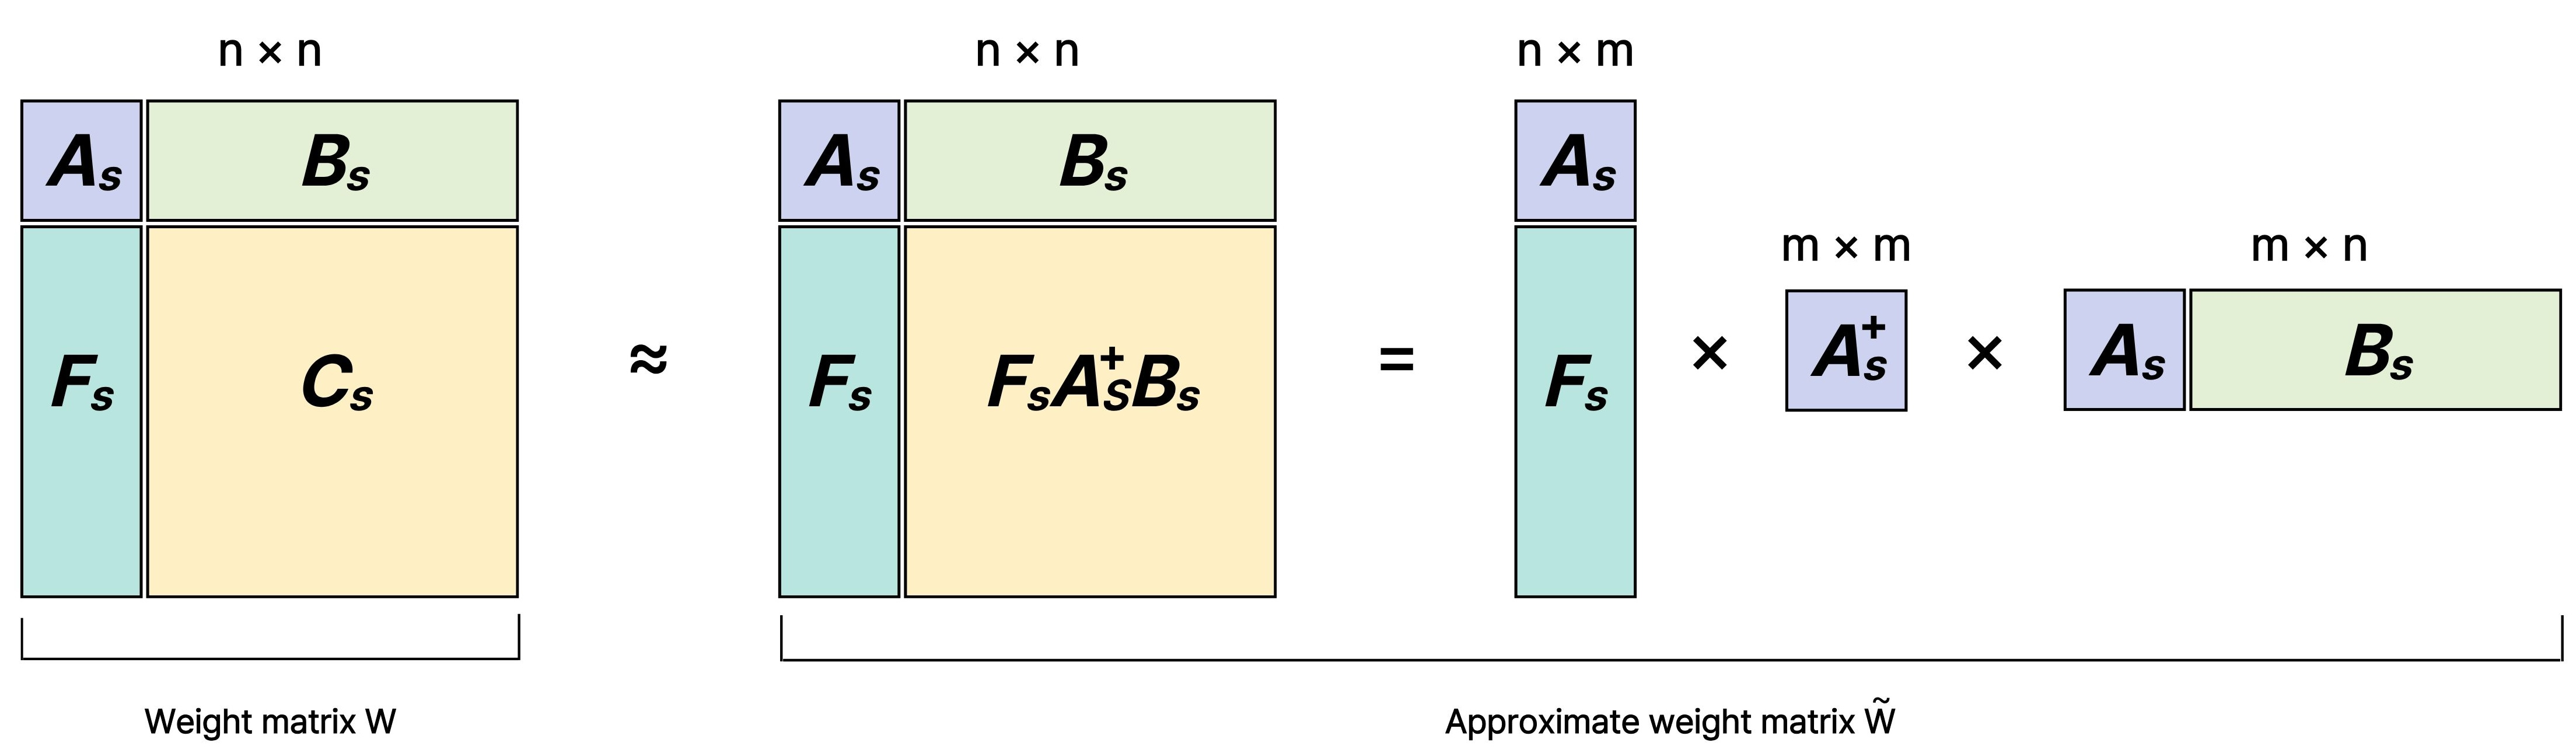
\includegraphics[width=0.49\textwidth]{../images/nystrom-approx.jpg}%
    }\quad
    \subfloat[Our $\scheme$ Freivald Algorithm\label{fig:zkdiet}]{%
        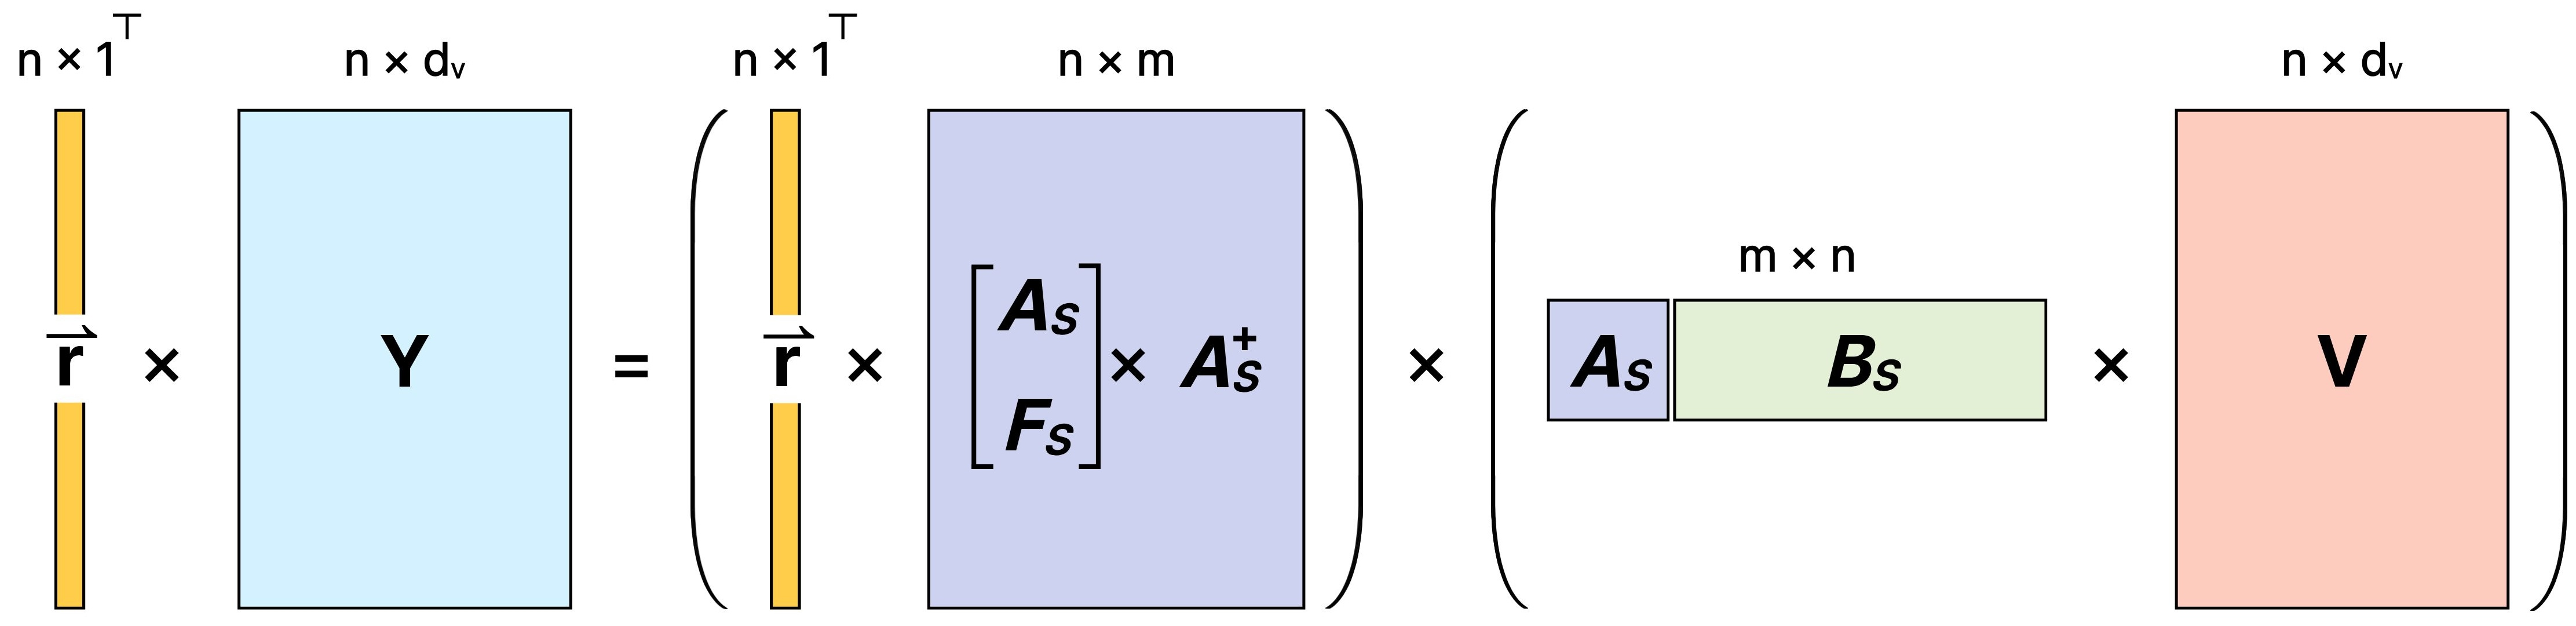
\includegraphics[width=0.49\textwidth]{../images/zkdiet-freivald.jpg}%
    }
    \caption{Low rank matrix multiplication with Freivald Algorithm}
\end{figure}

% 그림 1에서 보이듯이, 우리는 $n \times n$ 크기의 Self-attention 행렬을 직접 다루는 대신, 이를 $n \times m$, $m \times m$, $m \times n$ 형태의 저차원 행렬들로 분해하는 Nyströmformer의 절차를 수행한다. 이렇게 얻어진 Low-rank 표현에 대하여 Freivalds 알고리즘을 적용함으로써(그림 2), 검증 단계에서의 연산 부하를 $O(n^2)$에서 $O(mn)$ 수준인 $m(mn+d_v n)$ 크기의 벡터 곱으로 압축한다. 이를 통해 증명자(Prover)의 증명 생성 시간과 검증자(Verifier)의 오버헤드를 동시에 최소화할 수 있다.

As illustrated in Figure~\ref{fig:nystrom-approx}, rather than directly handling the $n \times n$ self-attention matrix, we follow the Nyströmformer procedure and decompose it into a sequence of low-dimensional matrices of shapes $n \times m$, $m \times m$, and $m \times n$. By applying Freivalds’ algorithm to this low-rank representation(in Figure~\ref{fig:zkdiet}), we compress the verification workload from $O(n^2)$ to $O(n)$, effectively reducing it to vector multiplications of size $n+m^3+nm^2+mnd_v+m^3+nmd_v$. This enables simultaneous reduction of both the prover’s proof-generation time and the verifier’s computational overhead.

% 이처럼 축소된 행렬곱을 Freivalds 알고리즘에 기반하여 검증하기 위해, 우리는 Commit-and-Prove SNARK (CP-SNARK) 구조를 채택한다. 먼저 어텐션 행렬은 회로 외부에서 커밋되고, 증명자는 커밋된 행렬이 회로 내부의 비공개 증인(witness)과 일관됨을 보이는 동시에, low-rank 근사 연산으로 얻어진 행렬곱 결과가 올바름을 저차원 근사에 최적화된  선형 복잡도의 Freivalds 검증을 통해 증명한다. 전체 어텐션 행렬 대신 외부에서 생성된 커밋먼트(commitment)만을 검증자에게 전달함으로써, 검증자는 상수 시간의 커밋 검증만 수행하면 된다. 이러한 설계는 대규모 모델에서 발생하는 행렬 연산에 대해, 증명 생성 비용과 검증 비용을 동시에 크게 감소시킨다.
% 영지식 회로는 유한체 위에서 동작하기 때문에, 실수 기반 Transformer 연산을 그대로 표현할 수 없다. 따라서 우리는 연산을 정밀도 손실을 최소화하는 방식으로 양자화하였으며, 이 과정에서 ZEN~\cite{…}에서 제안된 R1CS friendly quantization technique을 사용하였다.

\begin{figure*}[!ht]
    \centering
    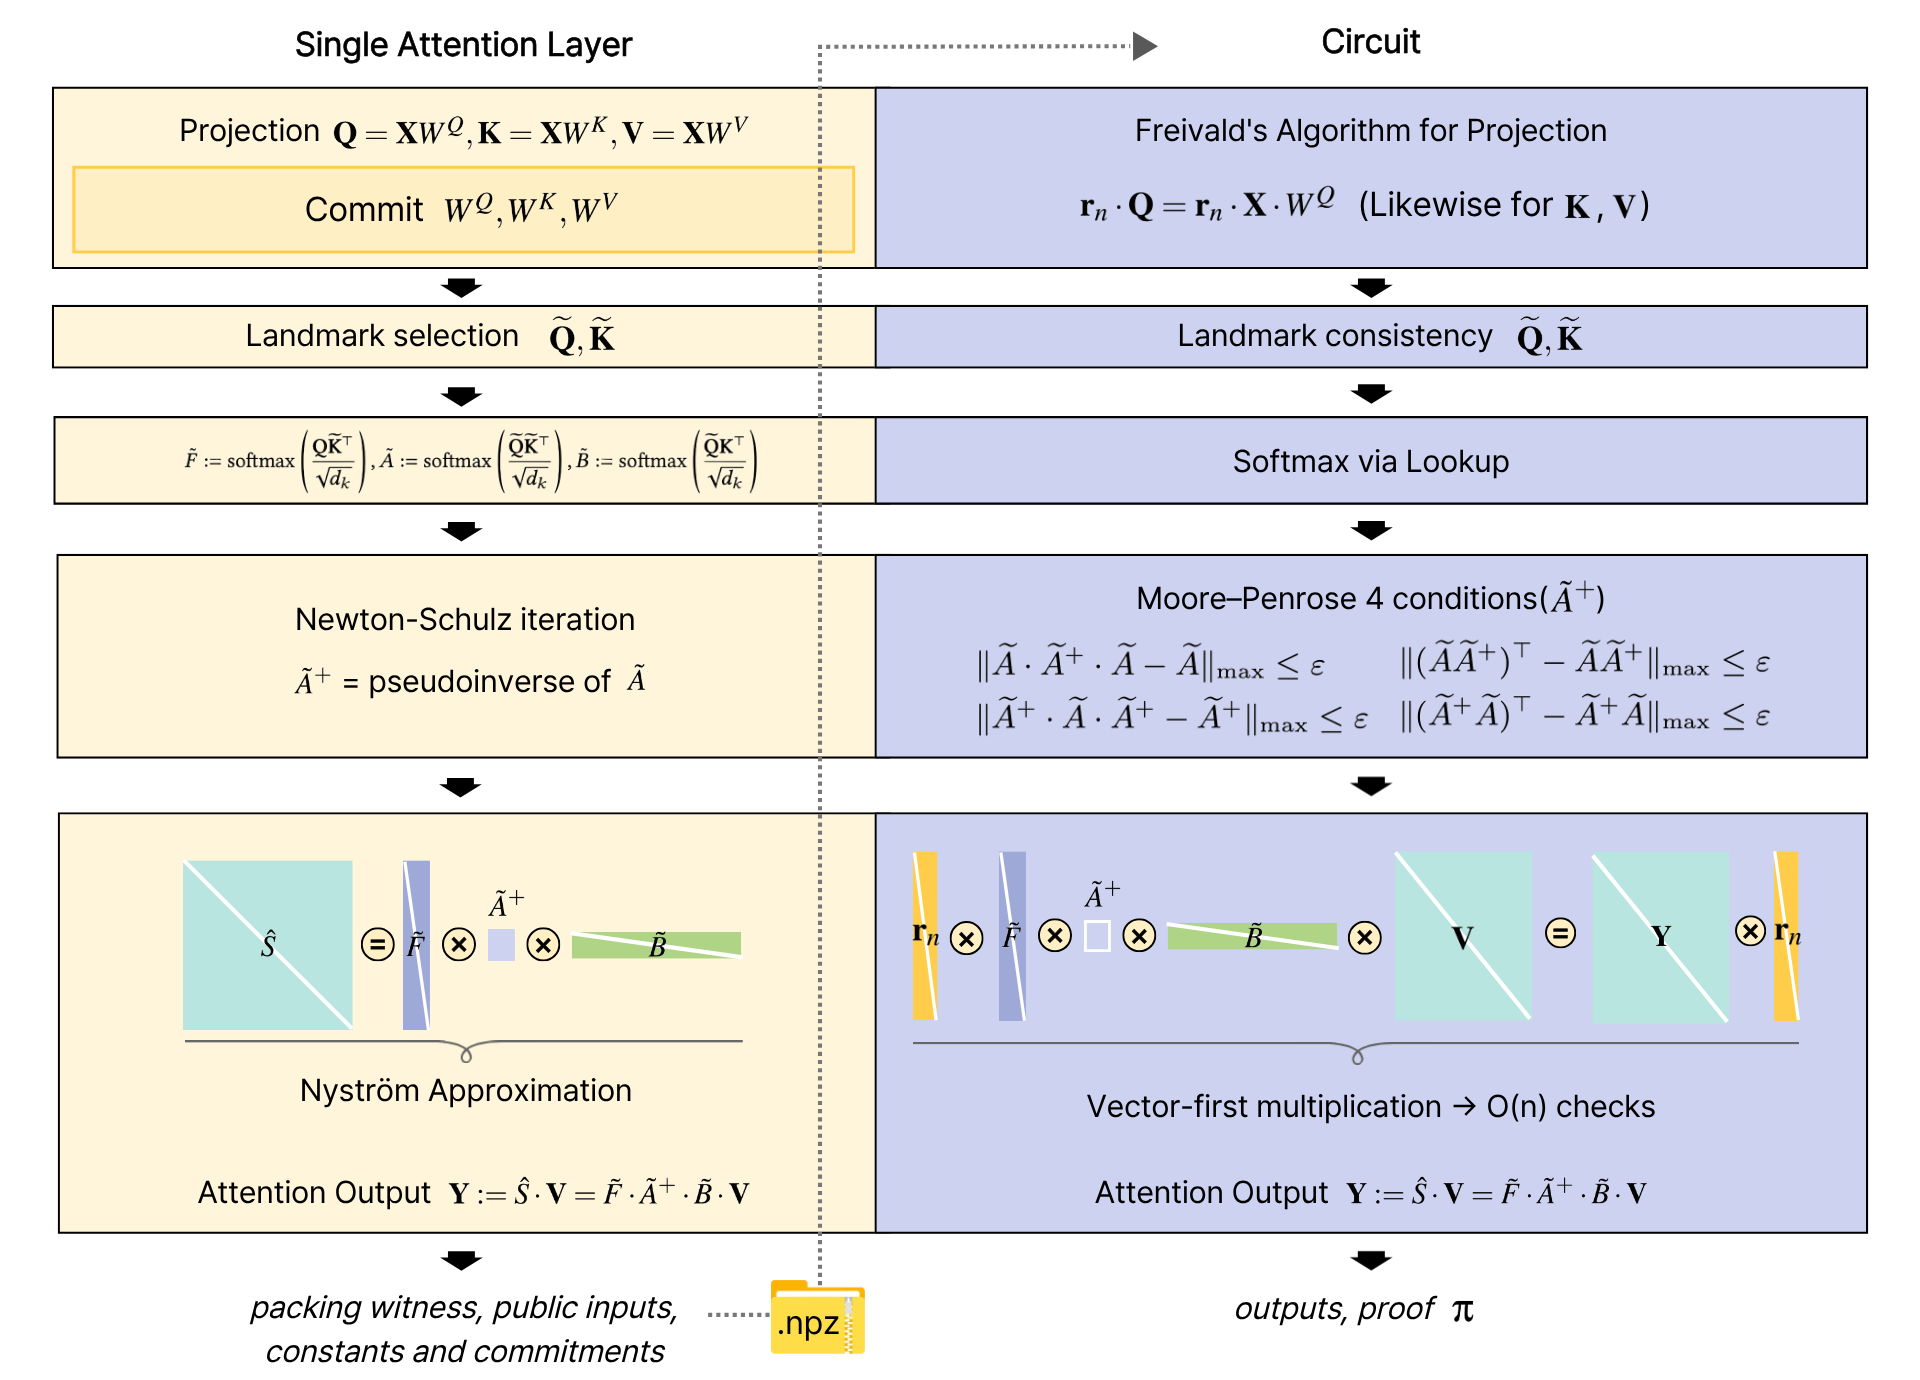
\includegraphics[width=0.6\linewidth]{../images/overview.png}
    \caption{Overview of Self-Attention and our framework}
    \label{fig:attention-overview}
\end{figure*}

To verify such low-rank matrix multiplications using Freivalds’ algorithm, we adopt a Commit-and-Prove SNARK (CP-SNARK) architecture. (in Figure~\ref{fig:attention-overview}) The attention matrix is first committed outside the circuit, and the prover shows that the committed matrix is consistent with the private witness inside the circuit, while simultaneously proving that the matrix multiplication result is correct via a Freivalds algorithm with linear complexity. Instead of transmitting the full attention matrix, only the externally generated commitment is provided to the verifier, who then performs merely constant-time commitment checks. This design substantially reduces both proving and verification costs for matrix operations arising in large-scale models.

Because zero-knowledge circuits operate over finite fields, real-valued Transformer computations cannot be represented directly. We therefore quantize the computations in a manner that minimizes precision loss, leveraging the R1CS-friendly quantization technique proposed in~\cite{ZEN}.



\begin{figure*}[!ht]
\center
\fbox{\procedure[head=\textbf{Protocol}, bodylinesep=2mm]{}{
        \mathcal{P}(\ck, \X; \{ W^Q, W^K, W^V\}) \< \< \mathcal{V}(\vk, \X) \\
        % \Q, \K, \V \gets \X\cdot W^Q, \X \cdot W^K, \X \cdot W^V \\
        \Q, \K, \V, \Q\widetilde{\K}^\top, \widetilde{\Q}\widetilde{\K}^\top, \widetilde{\Q}\K^\top, \widetilde{A}^+ \gets \NystromAttention(\X, W^Q, W^K, W^V) \\
        % \widetilde{\cm}_Q \gets \commit(\ck, \Q; \tilde{o_Q}) \\
        % \widetilde{\cm}_K \gets \commit(\ck, \K; \tilde{o_K}) \\
        % \widetilde{\cm}_V \gets \commit(\ck, \V; \tilde{o_V}) \\
        (\widetilde{\cm}_Q,\widetilde{\cm}_K, \widetilde{\cm}_V) \gets \commit(\ck,\Q;\tilde{o_Q}),\ \commit(\ck,\K;\tilde{o_K}),\ \commit(\ck,\V;\tilde{o_V}) \\
        \<  \sendmessageright*[2cm]{\widetilde{\cm}_Q, \widetilde{\cm}_K, \widetilde{\cm}_V} \< \\
        \< \sendmessageleft*[2cm]{\rand_n, \rand_k } \< \rand_n \sample \F^n, \t \rand_k \sample \F^k  \\
        \ins := \{ \X, \rand_n, \rand_k  \} \\
        \comwit := \{ \Q, \K, \V \} \\
        \uncomwit := \{ W^Q, W^K, W^V, \Q\widetilde{\K}^\top, \widetilde{\Q}\widetilde{\K}^\top, \widetilde{\Q}\K^\top, \widetilde{A}^+ \} \\
        \pi \gets \Pi_\cc.\prove(\pk, \ins; (\comwit, \uncomwit)) \\
        \<  \sendmessageright*[2cm]\pi \< \\
        \< \< \Pi_\cc.\verify(\vk, \ins, \widetilde{\cm}_Q, \widetilde{\cm}_K, \widetilde{\cm}_V, \pi)
    }}
    \caption{Our protocol}
    \label{fig:protocol}
\end{figure*}
%-------------------------------------------------------------------------------
\section{\name: Efficient Proofs of Low-Rank Matrix Multiplication via Freivalds' Algorithm}

%-------------------------------------------------------------------------------

In this section, we present the core protocol of \name. Our goal is to prove the correctness of \nystrom-approximated low-rank self-attention while avoiding any explicit computation of the $n \times n$ attention matrix inside the circuit. Concretely, we design the protocol so that the number of constraints scales linearly with the sequence length $n$. To this end, we adopt a commit-and-prove SNARK architecture that pushes computationally expensive operations (e.g., large matrix multiplications and pseudoinverse computation) outside the circuit, and proves only their correctness inside the circuit using a small number of constraints.


\subsection{Protocol Overview}
Our protocol follows the message flow shown in Figure~\ref{fig:protocol}.
First, the prover runs $\NystromAttention$ on the input sequence $\X \in \mathbb{F}^{n \times d}$ and the model parameters $W^Q, W^K, W^V \in \mathbb{F}^{d \times d}$.
This computation is performed outside the circuit, and thus can include heavy operations such as pseudoinverse computation. From this execution, the prover obtains the query, key, and value matrices $\Q,\K,\V$, where $\Q=\X W^Q$, $\K=\X W^K$, and $\V=\X W^V$. The prover then commits to $\Q,\K,\V$ and sends the resulting commitments $\widetilde{\cm}_Q, \widetilde{\cm}_K, \widetilde{\cm}_V$ to the verifier.

Next, the verifier samples random challenge vectors $\rand_n \in \F^n$ and $\rand_k \in \F^k$ for Freivalds' randomized checks, and sends them to the prover.
The prover sets the public instance as
\[
    \ins := (\X, \rand_n, \rand_k),
\]
and generates a SNARK proof $\pi$ using the proving key $\pk$.
The witness consists of a committed part
\[
    \comwit := (\Q,\K,\V),
\]
and an uncommitted part
\[
    \uncomwit := \bigl(W^Q, W^K, W^V,\; \Q\widetilde{\K}^{\top},\; \widetilde{\Q}\widetilde{\K}^{\top},\; \widetilde{\Q}\K^{\top},\; \widetilde{A}^{+}\bigr).
\]
Finally, the verifier checks the proof $\pi$ against the public instance $\ins$ and the previously received commitments
$\widetilde{\cm}_Q, \widetilde{\cm}_K, \widetilde{\cm}_V$ using the verification key $\vk$.
The above interactive protocol can be made non-interactive via the Fiat--Shamir transformation.




% \begin{algorithm}[h]
% \raggedright
% \scalebox{1}{
% \small
% \begin{minipage}{0.95\linewidth}
% \textbf{Input: } \text{model parameters } $W^Q, W^K, W^V \in \mathbb{F}^{d \times d}$ \\
% \textbf{Output: } commitments $\cm_Q, \cm_K, \cm_V$ \\[2pt]
% \underline{$\comparams(W^Q, W^K, W^V)$}: \\[2pt]
% \pseudocode[colspace,linenumbering]{
%   o_Q, o_K, o_V \sample \mathbb{F} \\
%   \cm_Q \gets \ped.\commit(\ck, W^Q; o_Q) \\
%   \cm_K \gets \ped.\commit(\ck, W^K; o_K) \\
%   \cm_V \gets \ped.\commit(\ck, W^V; o_V) \\
%   \pcreturn (\cm_Q, \cm_K, \cm_V)
% }
% \end{minipage}
% }
% \caption{Commit model parameters}
% \label{algo:commit}
% \end{algorithm}

\subsection{\nystrom-Based Low-Rank Self-Attention}
Our system adopts a \nystrom-based low-rank approximation for self-attention. In \nystromformer, the query and key matrices are represented using $k$ landmark vectors.
Algorithm~\ref{alg:landmark} describes the landmark selection procedure. Given $\Q=[\mathbf{q}_1,\ldots,\mathbf{q}_n]$ and $\K=[\mathbf{k}_1,\ldots,\mathbf{k}_n]$, We summarize the length-$n$ sequence using $k$ landmarks by partitioning it into $k$ consecutive segments of length $\ell = n/k$ and defining each landmark as the average over the $\ell$ tokens in its segment. This yields $\widetilde{\Q}=[\tilde{\mathbf{q}}_1,\ldots,\tilde{\mathbf{q}}_k]$ and $\widetilde{\K}=[\tilde{\mathbf{k}}_1,\ldots,\tilde{\mathbf{k}}_k]$. 
With these landmarks, we avoid constructing the full $n\times n$ attention matrix and instead decompose the computation into three lower-dimensional matrices: $\Q\widetilde{\K}^{\top} \in \mathbb{F}^{n \times k}, \widetilde{\Q}\widetilde{\K}^{\top} \in \mathbb{F}^{k \times k}, \widetilde{\Q}\K^{\top} \in \mathbb{F}^{k \times n}$
% an $n\times k$ matrix $\Q\widetilde{\K}^{\top}$, a $k\times k$ matrix $\widetilde{\Q}\widetilde{\K}^{\top}$, and a $k\times n$ matrix $\widetilde{\Q}\K^{\top}$.

We then apply the row-wise softmax to each of these matrices and compute
\[
\tilde{F} := \sfmax\!\Bigl(\tfrac{\Q\widetilde{\K}^{\top}}{\sqrt{d}}\Bigr),
\tilde{A} := \sfmax\!\Bigl(\tfrac{\widetilde{\Q}\widetilde{\K}^{\top}}{\sqrt{d}}\Bigr),
\tilde{B} := \sfmax\!\Bigl(\tfrac{\widetilde{\Q}\K^{\top}}{\sqrt{d}}\Bigr).
\]
Here, $\tilde{A}$ is a small $k\times k$ matrix corresponding to the landmark submatrix of the original $n \times n$ attention matrix.
Overall, the combination of $\tilde{F}$, $\tilde{A}$, and $\tilde{B}$ yields a \nystrom\ approximation of the full attention map.

Finally, we compute an approximation to the Moore--Penrose pseudoinverse $\tilde{A}^{+}$ of the $k\times k$ matrix $\tilde{A}$. While one could compute $\tilde{A}^{+}$ via SVD, this is typically inefficient on GPU hardware. Therefore, \nystromformer\ approximates $\tilde{A}^{+}$ via an iterative polynomial approximation to the SVD. Algorithm~\ref{alg:inverse} shows this iterative procedure. 

Using the resulting $\tilde{A}^{+}$, we form the final approximated attention matrix
\[
    \hat{S} := \tilde{F}\cdot \tilde{A}^{+}\cdot \tilde{B},
\]
and compute the attention output as
\[
    \Y := \hat{S} \cdot \V.
\]
Algorithm~\ref{alg:nystromAttention} provides the complete \nystrom-based self-attention computation used in our framework.

\begin{algorithm}[t!]
\raggedright
\scalebox{1}{
\small
\begin{minipage}{0.95\linewidth}
\textbf{Input: } $\text{Query }\Q \text{ and Key } \K \in \mathbb{F}^{n \times d}$ \\
\textbf{Output: } \text{Landmark points } $\widetilde{\Q}, \widetilde{\K} \in \mathbb{F}^{k \times d}$  \\[2pt]
\underline{$\selectLandmarks(\Q, \K)$:}\\[2pt]
\pseudocode[colspace,linenumbering]{
    \pcparse \Q = [\mathbf{q}_1, \mathbf{q}_2, \dots, \mathbf{q}_n], \K = [\mathbf{k}_1, \mathbf{k}_2, \dots, \mathbf{k}_n] \\
    \ell \gets n / k \\
    \pcfor j \in \{ 1, \dots, k\} \pcdo \\
        \t \tilde{\mathbf{q}}_j \gets \sum_{i=(j-1) \times \ell + 1}^{j\ell} \frac{\mathbf{q}_i}{\ell}, \tilde{\mathbf{k}}_j \gets \sum_{i=(j-1) \times \ell + 1}^{j\ell} \frac{\mathbf{k}_i}{\ell} \\
    \pcendfor \\
    \widetilde{\Q} \gets [\tilde{\mathbf{q}}_1, \tilde{\mathbf{q}}_2, \dots, \tilde{\mathbf{q}}_k] \\
    \widetilde{\K} \gets [\tilde{\mathbf{k}}_1, \tilde{\mathbf{k}}_2, \dots, \tilde{\mathbf{k}}_k] \\
    \pcreturn (\widetilde{\Q}, \widetilde{\K})
}
\end{minipage}
}
\caption{Select landmarks}
\label{alg:landmark}
\end{algorithm}


\begin{algorithm}[t!]
\raggedright
\scalebox{1}{
\small
\begin{minipage}{0.95\linewidth}
\textbf{Input: } $\text{selected landmark matrix } \tilde{A} \in \mathbb{F}^{k \times k}$\\
\textbf{Output: } $\text{approximate pseudoinverse }\tilde{A}^+ \in \mathbb{F}^{k \times k}$\\[2pt]
\underline{$\computeMPInverse(\tilde{A})$}: \\[2pt]
\pseudocode[colspace,linenumbering]{
  Z_0 \gets \tilde{A}^\top / \left(\|\tilde{A}\|_1 \cdot \|\tilde{A}\|_\infty\right) \\
  \text{Set } T \text{ (e.g., } T=6 \text{ iterations)} \\
  \pcfor t \in \{0,\dots,T-1\} \pcdo \\
    \t Z_{t+1} \gets \frac{1}{4} Z_t \Big( 13I - \tilde{A}Z_t\big(15I - \tilde{A}Z_t(7I - \tilde{A}Z_t)\big) \Big) \\
  \pcendfor \\
  \tilde{A}^+ \gets Z_T \\
  \pcreturn \tilde{A}^+
}
\end{minipage}
}
\caption{Compute Moore--Penrose inverse}
\label{alg:inverse}
\end{algorithm}


% \begin{algorithm}[!t]
% \raggedright
% \scalebox{1}{
% \small
% \begin{minipage}{0.95\linewidth}
% \noindent
% \begin{tabular}{@{}l l@{}}
% \textbf{Input:} &
% \text{Input sequence } $\X \in \mathbb{F}^{n \times d}$, \\
% & \text{Model parameters } $W^Q, W^K, W^V \in \mathbb{F}^{d \times d}$ \\

% \textbf{Output:} &
% \text{Attention matrix } $\Y := \hat{\mathbf{S}}\mathbf{V} \in \mathbb{F}^{n \times d}$, \\
% & \text{Auxiliary } $\textit{aux} := \Q, \K, \V, \Q\widetilde{\K}^\top, \widetilde{\Q}\widetilde{\K}^\top, \widetilde{\Q}\K^\top, \widetilde{A}^+$ \\[2pt]
% \end{tabular}

% \underline{$\NystromAttention(\X, W^Q, W^K, W^V)$}: \\[2pt]
% \pseudocode[colspace,linenumbering]{
%     \text{Compute } \Q, \K, \V \in \mathbb{F}^{n \times d}: \\
%         \t \Q := \X \cdot W^Q \\
%         \t \K := \X \cdot W^K \\ 
%         \t \V := \X \cdot W^V \\[2pt]
%     \text{Select landmarks:} \\
%         \t \widetilde{\Q}, \widetilde{\K} \gets \selectLandmarks(\Q, \K) \\ [2pt]
%     \text{Compute approximation for the attention matrix: } \\
%         \t \tilde{F} := \sigma\left(\frac{\Q\widetilde{\K}^\top}{\sqrt{d}}\right) \\
%         \t \tilde{A} := \sigma\left( \frac{\widetilde{\Q}\widetilde{\K}^\top}{\sqrt{d}} \right) \\
%         \t \tilde{B} := \sigma\left(\frac{\widetilde{\Q}\K^\top}{\sqrt{d}}\right) \\
%     \text{Compute Moore-Penrose inverse } \tilde{A}^+: \\
%         \t \tilde{A}^+ \gets \computeMPInverse(\tilde{A}) \\
%     \hat{S} := \tilde{F} \cdot \tilde{A}^+ \cdot \tilde{B} \\
%     \text{Compute } \mathbf{Y}\\
%         \t \Y := \hat{S} \cdot \V = \tilde{F} \cdot \tilde{A}^+ \cdot \tilde{B} \cdot \V \\
%     \textit{aux} := \Q, \K, \V, \Q\widetilde{\K}^\top, \widetilde{\Q}\widetilde{\K}^\top, \widetilde{\Q}\K^\top, \widetilde{A}^+ \\
%     \pcreturn \Y, \textit{aux}
% }
% \end{minipage}
% }
% \caption{\nystrom\ approximation of attention matrix}
% \label{alg:nystromAttention}
% \end{algorithm}

\begin{algorithm}[!t]
\raggedright
\scalebox{1}{
\small
\begin{minipage}{0.95\linewidth}
\noindent
\begin{tabular}{@{}l l@{}}
\textbf{Input:} &
\text{Input sequence } $\X \in \mathbb{F}^{n \times d}$, \\
& \text{Model parameters } $W^Q, W^K, W^V \in \mathbb{F}^{d \times d}$ \\

\textbf{Output:} &
\text{Attention matrix } $\Y := \hat{\mathbf{S}}\mathbf{V} \in \mathbb{F}^{n \times d}$, \\
& \text{Auxiliary } $\textit{aux} := \Q, \K, \V, \Q\widetilde{\K}^\top, \widetilde{\Q}\widetilde{\K}^\top, \widetilde{\Q}\K^\top, \widetilde{A}^+$ \\[2pt]
\end{tabular}

\underline{$\NystromAttention(\X, W^Q, W^K, W^V)$}: \\[2pt]
\pseudocode[colspace,linenumbering]{
    % \text{Compute } \Q, \K, \V \in \mathbb{F}^{n \times d}: \\
    \Q := \X \cdot W^Q \\
    \K := \X \cdot W^K \\ 
    \V := \X \cdot W^V \\[2pt]
    % \text{Select landmarks:} \\
    \widetilde{\Q}, \widetilde{\K} \gets \selectLandmarks(\Q, \K) \\ [2pt]
    % \text{Compute approximation for the attention matrix: } \\
    \tilde{F} := \sigma\left(\frac{\Q\widetilde{\K}^\top}{\sqrt{d}}\right), \tilde{A} := \sigma\left( \frac{\widetilde{\Q}\widetilde{\K}^\top}{\sqrt{d}} \right), \tilde{B} := \sigma\left(\frac{\widetilde{\Q}\K^\top}{\sqrt{d}}\right) \\
    % \text{Compute Moore-Penrose inverse } \tilde{A}^+: \\
    \tilde{A}^+ \gets \computeMPInverse(\tilde{A}) \\
    \hat{S} := \tilde{F} \cdot \tilde{A}^+ \cdot \tilde{B} \\
    % \text{Compute } \mathbf{Y}\\
    \Y := \hat{S} \cdot \V = \tilde{F} \cdot \tilde{A}^+ \cdot \tilde{B} \cdot \V \\
    \textit{aux} := \Q, \K, \V, \Q\widetilde{\K}^\top, \widetilde{\Q}\widetilde{\K}^\top, \widetilde{\Q}\K^\top, \widetilde{A}^+ \\
    \pcreturn \Y, \textit{aux}
}
\end{minipage}
}
\caption{\nystrom\ approximation of attention matrix}
\label{alg:nystromAttention}
\end{algorithm}


\subsection{Efficient Verification via Freivalds’ Algorithm}
Our protocol uses Freivalds’ algorithm as a core tool to efficiently verify that the low-rank self-attention computation is performed correctly. In particular, within the zk-SNARK circuit, we employ Freivalds’ algorithm to ensure that the following key operations can be verified with linear cost. \\

\sss{Query/Key/Value matrix generation}
Using the verifier's random vector $\rand_n$, we check the relation $\Q = \X W^Q$ by comparing $\rand_n^{\top} \Q$ with $\rand_n^{\top}(\X W^Q)$.
We verify $\K$ and $\V$ in the same way. Rather than proving the full $n\times d$ matrix product directly, this Freivalds' check reduces verification to computing only the vector-matrix product $\rand_n^{\top}\X W^Q$, thereby reducing the complexity to $\mathcal{O}(n)$. \\

\sss{Low-rank matrix operations}
We also verify low-dimensional products such as $\Q\widetilde{\K}^{\top}$,
$\widetilde{\Q}\widetilde{\K}^{\top}$, and $\widetilde{\Q}\K^{\top}$
by multiplying each matrix with a random vector of matching dimension,
i.e., $\rand_n$ or $\rand_k$.
For instance, we can certify the correctness of $\Q\widetilde{\K}^{\top}$ by checking the following equality:
\[
\rand_n^{\top}\!\bigl(\Q\widetilde{\K}^{\top}\bigr)
\stackrel{?}{=}
(\rand_n^{\top}\Q)\,\widetilde{\K}^{\top}
\]

Similarly, the products $\widetilde{\Q}\widetilde{\K}^{\top}$ and $\widetilde{\Q}\K^{\top}$ are validated with linear cost, without explicitly computing the full matrix multiplications inside the circuit. \\

\sss{Moore--Penrose pseudoinverse}
Computing the Moore--Penrose pseudoinverse $\tilde{A}^{+}$ inside the circuit is inefficient.
Instead, we certify that $\tilde{A}^{+}$ is the pseudoinverse of $\tilde{A}$ by checking the four
Moore--Penrose conditions, which correspond to lines~19--22 in Figure~\ref{fig:relation}:
\begin{itemize}
    \item $\tilde{A}\cdot\tilde{A}^{+}\cdot\tilde{A}=\tilde{A}$
    \item $\tilde{A}^{+}\cdot\tilde{A}\cdot\tilde{A}^{+}=\tilde{A}^{+}$
    \item $(\tilde{A}\tilde{A}^{+})^{\top}=\tilde{A}\tilde{A}^{+}$
    \item $(\tilde{A}^{+}\tilde{A})^{\top}=\tilde{A}^{+}\tilde{A}$
\end{itemize}
This allows the prover to efficiently demonstrate that $\tilde{A}^{+}$ is a valid Moore--Penrose pseudoinverse of $\tilde{A}$ without explicitly computing it in-circuit.

The relations that the prover must satisfy are formalized in Figure~\ref{fig:relation} as the definition of the circuit relation. In particular, the relation $\R(\ins,\wit)$ takes the public instance $\ins=(\X,\rand_n,\rand_k)$ and the witness $\wit=(\Q,\K,\V, W^Q, W^K, W^V, \Q\widetilde{\K}^\top, \widetilde{\Q}\widetilde{\K}^\top, \widetilde{\Q}\K^\top, \widetilde{A}^+)$, and enforces all required equalities as well as the softmax computation. All key equalities are expressed in the form of products with the random vectors, accordingly, the circuit computes only vector inner products.


\begin{figure}[t!]
\center
\fbox{\procedure[
    head=\textbf{Relation},
    bodylinesep=2mm,
    linenumbering,
    mode=text
]{}{
        $\R(\ins, \wit): $\\[2pt]
        $\t \pcparse \ins = (\X, \rand_n, \rand_k), \wit = (\comwit, \uncomwit)$ \\
        $\t \pcparse \comwit = (\Q, \K, \V)$ \\
        $\t \pcparse \uncomwit = (W^Q, W^K, W^V, \Q\widetilde{\K}^\top, \widetilde{\Q}\widetilde{\K}^\top, \widetilde{\Q}\K^\top, \widetilde{A}^+)$ \\
        $\t \pcparse \Q = [\mathbf{q}_1, \mathbf{q}_2, \dots, \mathbf{q}_n], \K = [\mathbf{k}_1, \mathbf{k}_2, \dots, \mathbf{k}_n]$ \\
        $\t \rand_n \cdot \Q = \rand_n \cdot \X \cdot W^Q$ \\
        $\t \rand_n \cdot \K = \rand_n \cdot \X \cdot W^K$ \\
        $\t \rand_n \cdot \V = \rand_n \cdot \X \cdot W^V$ \\
        $\t \pcfor j \in \{ 1, \dots, k\} \pcdo$ \\
            $\t \t\tilde{\mathbf{q}}_j \gets \sum_{i=(j-1) \times \ell + 1}^{j\ell}  \frac{\mathbf{q}_i}{\ell}, \t
            \tilde{\mathbf{k}}_j \gets \sum_{i=(j-1) \times \ell + 1}^{j\ell} \frac{\mathbf{k}_i}{\ell}$ \\
        $\t \pcendfor$ \\
        $\t \widetilde{\Q} \gets [\tilde{\mathbf{q}}_1, \dots, \tilde{\mathbf{q}}_k], \widetilde{\K} \gets [\tilde{\mathbf{k}}_1, \dots, \tilde{\mathbf{k}}_k]$ \\
        $\t \rand_n \cdot \Q\widetilde{\K}^\top = \rand_n \cdot \Q \cdot \widetilde{\K}^\top$ \\
        $\t \rand_k \cdot \widetilde{\Q}\widetilde{\K}^\top = \rand_k \cdot \widetilde{\Q} \cdot \widetilde{\K}^\top$ \\
        $\t \rand_n \cdot \widetilde{\Q}\K^\top = \rand_n \cdot \widetilde{\Q} \cdot \K^\top$ \\
        $\t \widetilde{F} = \sigma\left( \frac{\Q\widetilde{\K}^\top}{\sqrt{d}} \right)$ \\
        $\t \widetilde{A} = \sigma\left( \frac{\widetilde{\Q}\widetilde{\K}^\top}{\sqrt{d}} \right)$ \\
        $\t \widetilde{B} = \sigma\left( \frac{\widetilde{\Q}\K^\top}{\sqrt{d}} \right)$ \\
        $\t \rand_k \cdot \widetilde{A} \cdot \widetilde{A}^+ \cdot \widetilde{A} = \rand_k \cdot \widetilde{A}$ \\
        $\t \rand_k \cdot \widetilde{A}^+ \cdot \widetilde{A} \cdot \widetilde{A}^+ = \rand_k \cdot \widetilde{A}^+$ \\
        $\t \rand_k \cdot (\widetilde{A}\widetilde{A}^+)^\top = \rand_k \cdot \widetilde{A}\widetilde{A}^+$ \\
        $\t \rand_k \cdot (\widetilde{A}^+\widetilde{A})^\top = \rand_k \cdot \widetilde{A}^+\widetilde{A}$ \\
        $\t \rand_n \cdot \Y = \rand_n \cdot \widetilde{F} \cdot \widetilde{A}^+ \cdot \widetilde{B} \cdot \V$ 
}}
\caption{Relation of \name}
\label{fig:relation}
\end{figure}





%-------------------------------------------------------------------------------
\section{Security}
\label{sec:figs}
%-------------------------------------------------------------------------------
% 해당 섹션에서, 우리는 zkDietFormer가 completeness와 security requirements를 만족함을 보일 것이다. zkDietFormer는 기반이 되는 CC-Groth16 프로토콜의 특성을 상속받아 완전성, 건전성, 그리고 영지식성을 보장한다.
In this section, we show that zkDietFormer satisfies the completeness and security requirements. Since zkDietFormer is built upon the cc-Groth16 protocol, it inherits its guarantees of completeness, soundness, and zero-knowledge.
\sss{Completeness} 
% 정직한 증명자가 Nystromformer 기반의 리니어 어텐션 연산을 충실히 수행하고 증명을 생성했다면, 검증자는 이를 항상 수용한다. 본 시스템에서 완전성 오류가 발생할 수 있는 지점은 룩업 테이블을 통한 비선형 연산(지수 함수)이다. 행렬 연산의 경우 프리발드 알고리즘은 수식이 올바를 때 항상 참을 반환한다. 룩업 테이블의 경우, 이론적으로 분모가 0이 될 가능성이 존재하나, zkDiet는 양자화 과정에서 zero-point 조정을 통해 모든 입력값을 양수 영역으로 매핑함으로써 분모가 0으로 근사되어 검증이 실패할 확률을 수학적으로 배제한다.
If an honest prover correctly performs the Nyströmformer-based linear attention computation and generates a proof, then the verifier always accepts it. In our system, the only potential source of completeness error arises from nonlinear operations handled via lookup tables (i.e., exponentiation operations). For matrix operations, the Freivalds’ algorithm always returns true when the equation is correct. In the case of lookup tables, one may theoretically consider situations where the denominator becomes zero. However, $\scheme$ avoids this issue through quantization with zero-point adjustment, which maps all inputs into the positive domain. As a result, any scenario in which the denominator is approximated as zero is mathematically eliminated, preserving completeness.


\sss{Soundness}
% 어떤 malicious한 prover이더라도 부정확한 행렬값 결과에 대하여 negl한 확률을 제외하고 verifier를 속일 수 없다. 우리의 시스템은 두가지 중요한 시큐리티 특성을 만족한다. 첫번째로. 행렬곱 $AB=C$의 무결성은 프리발드 알고리즘에 의해 보장되며, $AB \neq C$임에도 불구하고 랜덤 벡터 $x$에 대해 $ABx = Cx$가 성립할 확률은 유한체 $\mathbb{F}$의 크기에 반비례하는 $O(1/|\mathbb{F}|)$로 극히 낮다. 
Even a malicious prover cannot convince the verifier of an incorrect matrix computation except with negligible probability. Our system satisfies two essential security properties.

First, the integrity of the matrix multiplication $AB = C$ is guaranteed by Freivalds’ algorithm. When $AB \neq C$, the probability that a randomly chosen vector $r$ satisfies $ABx = C$ is extremely small, bounded by $O(1/|\mathbb{F}|)$, which is inversely proportional to the size of the finite field $\mathbb{F}$. To simplify the analysis, we assume in the following proof that the random vector $r$ used in Freivalds’ algorithm is sampled from the binary domain $\{0,1\}^n$.
%%%%%
\begin{proof}
% notation 수정 버전
Since $\hat{D}^{-1}$ is a diagonal matrix, the overall complexity $O(nkd)$ is determined by the $\mathbf{\tilde F{A'}^+}((\mathbf{B}^{'})^\top \mathbf{V})$ computation, excluding the cost of forming $\hat{D}^{-1}$. In the following section, we demonstrate that the Freivalds’ algorithm correctly verifies the computation of $\mathbf{\tilde F{A'}^+}((\mathbf{B}^{'})^\top \mathbf{V})$. Suppose the prover outputs a matrix $y'$ that has a different \textbf{structure or value} from the correct output $y=\mathbf{\tilde F{A'}^+}((\mathbf{B}^{'})^\top \mathbf{V})$.
Let
\[
  s_1' = \vec{r}\ y', \qquad
  s_2 = (\vec{r}\ \mathbf{\tilde F{A'}^+})((\mathbf{B}^{'})^\top \mathbf{V}).
\]
where $\mathbf{\tilde F{A'}^+},\mathbf{B}^{'} \in \mathbb{R}^{n\times k}, \mathbf{V} \in \mathbb{R}^{n\times d}, \vec{r} \in \{0,1\}^n$.
% 새로운 값들로 프리발드 알고리즘이 성립할 확률.
Let $\epsilon$ denote the error probability that the Freivalds verification outputs TRUE even when it is incorrect. We claim that if $\mathbf{\tilde F{A'}^+} \times ((\mathbf{B}^{'})^\top)\mathbf{V} = y'$, then $\epsilon = 0$, and if $\mathbf{\tilde F{A'}^+} \times ((\mathbf{B}^{'})^\top)\mathbf{V} \neq y'$, then $\epsilon \leq \frac{1}{2}$.
\begin{itemize}
    \item \textbf{Case $\mathbf{\tilde F{A'}^+}((\mathbf{B}^{'})^\top \mathbf{V})=y'$ :} The error matrix $D= \mathbf{\tilde F{A'}^+}((\mathbf{B}^{'})^\top \mathbf{V}) -y'$ is $0_{n\times d}$. Regardless of the choice of the vector $\vec{r}$, the equality is always satisfied because $\vec{r}D=\vec{0}$. Hence, 
    \[ \label{neqzero}
    \begin{split}
        \epsilon = \text{Pr}[\vec{r}D\neq 0] = \text{Pr}[\vec{r}0\neq \vec{0}] = 0
    \end{split}
    \]
    Therefore, the probability of error is $\epsilon=0$.
    \item \textbf{Case $\mathbf{\tilde F{A'}^+}((\mathbf{B}^{'})^\top \mathbf{V})\neq y'$ : } Let $\vec{P} = \vec{r}D= (p_1,p_2,...,p_d)$, where $D = \mathbf{\tilde F{A'}^+}((\mathbf{B}^{'})^\top \mathbf{V}) - y'.$ Since $\mathbf{\tilde F{A'}^+}((\mathbf{B}^{'})^\top \mathbf{V})\neq y'$, there exists at least one nonzero element in $D$. Let $d_{i^*,j}$ be the first nonzero entry in column $j$. For the value $\Delta=\sum_{k\neq i^*} r_kd_{kj}$. Using Bayes' Theorem, we can partition over $\Delta$.

    \begin{equation}\label{eq:pj}
    p_j = \sum_{k=1}^n r_k d_{kj}  
        = r_{i^*} d_{i^* j} + \sum_{k\neq i^*} r_k d_{kj} 
        = r_{i^*} d_{i^* j} + \Delta.
    \end{equation}

    \begin{equation}\label{eq:prob}
    \begin{aligned}
    \Pr[p_j=0] &= \Pr[p_j=0|\Delta=0]\cdot \Pr[\Delta=0] \\
               &\quad + \Pr[p_j=0|\Delta\neq0]\cdot \Pr[\Delta\neq 0].
    \end{aligned}
    \end{equation}

    \begin{equation}\label{eq:half}
    \Pr[p_j=0|\Delta=0] = \Pr[r_{i^*}=0] = \frac{1}{2}.
    \end{equation}

    For $\text{Pr}[p_j=0|\Delta\neq0]$, if $r_{i^*}d_{i^*j} + \Delta = 0$, it holds as long as $r_{i^*}=1$ (among the possible values of $r_{i^*} \in \{0,1\}$)so 
    
    \[
        \text{Pr}[p_j=0|\Delta\neq0] = \Pr[r_{i^*}=1] = \frac{1}{2}
    \]
        
    if $d_{i^*j} + \Delta \neq 0$, then $r_{i^*}$ cannot take any value to satisfy the condition, so $\text{Pr}[p_j=0|\Delta\neq0] = 0$. Therefore, $\text{Pr}[p_j=0|\Delta\neq0] \le \frac{1}{2}$.

    After taking this case into account, the probability can be rewritten as follows:

    \begin{equation}\label{neqzero2-1}
        \begin{aligned}
        \Pr[p_j=0] 
        &\leq \frac{1}{2} \cdot \Pr[\Delta=0] 
           + \frac{1}{2} \cdot \Pr[\Delta\neq 0] \\
        &= \frac{1}{2} \cdot \Pr[\Delta=0] 
           + \frac{1}{2} \cdot (1-\Pr[\Delta=0]) \\
        &= \frac{1}{2}.
        \end{aligned}
    \end{equation}

    \begin{equation}\label{neqzero2-2}
        \epsilon = \Pr[\vec{P}=0 \mid y' \neq y].
    \end{equation}

    \begin{equation}\label{neqzero2-3}
    \begin{aligned}
        \epsilon 
        &= \Pr[\vec{P}=0] \\
        &= \Pr[p_1=0 \wedge \cdots \wedge p_j=0 \wedge \cdots \wedge p_d=0] \\
        &\leq \Pr[p_j=0] \leq \frac{1}{2}.
    \end{aligned}
    \end{equation}

    \begin{equation}\label{neqzero2-4}
        \epsilon \leq \frac{1}{2}.
    \end{equation}
\end{itemize}

After $t$ independent repetitions, the $\epsilon$ becomes $(\frac{1}{2})^t$, which is negligible in $t$. Therefore, the verification protocol is sound: the probability that it outputs TRUE when $\mathbf{\tilde F{A'}^+}((\mathbf{B}^{'})^\top \mathbf{V})\neq y'$ is $\epsilon \leq (\frac{1}{2})^t$.
\end{proof}
%%%%%
% 둘째, KZG 다항식 커밋먼트의 강한 바인딩(binding) 속성으로 인해, 증명자는 커밋된 값과 다른 값을 주장할 수 없다. 우리는 CP-SNARK의 commit-and-prove 특성을 통해 (1) 행렬곱의 정당성, (2) Softmax 결과의 일치성을 증명하고, cp-link를 활용하여 (3) 두 연산 간 입력 데이터의 일관성까지 함께 보장한다. 따라서 커밋된 값이 다른 값으로 교체되는 경우, 검증을 통과하는 것은 불가능하다.
Second, the strong binding property of the KZG polynomial commitment ensures that the prover cannot claim values different from those already committed. Using the commit-and-prove capability of CP-SNARK, we prove (1) correctness of matrix multiplication and (2) consistency of the Softmax outputs, while cp-link additionally guarantees (3) input consistency across these two computations. Consequently, any attempt to replace a committed value with another one cannot pass verification.


\sss{Zero-Knowledge}
% zkDiet는 추론 과정에서 모델 가중치, 입력값, 중간 활성값을 포함한 어떠한 비밀 정보도 외부에 노출하지 않는다. 모든 값은 커밋먼트 형태로 처리되며, 검증자는 오직 리니어 트랜스포머 계산의 올바름만을 확인할 수 있을뿐, 커밋먼트 내부의 실제 값에 대해서는 어떠한 추가 정보(no additional information)도 얻을 수 없다
$\scheme$ reveals no secret information during inference, including model weights, inputs, or intermediate activations. All values are handled in committed form. The verifier learns only that the linear transformer computation was carried out correctly, while gaining no additional information about the committed values.
%-------------------------------------------------------------------------------
\section{Experiments}
%-------------------------------------------------------------------------------







%-------------------------------------------------------------------------------
\section*{Acknowledgments}
%-------------------------------------------------------------------------------
The USENIX latex style is old and very tired, which is why
there's no \textbackslash{}acks command for you to use when
acknowledging. Sorry.

\textbf{Do not include any acknowledgements in your submission which may deanonymize you (e.g., because of specific affiliations or grants you acknowledge)}
%-------------------------------------------------------------------------------
% optional clearing of the page
\cleardoublepage
\appendix
\section*{Ethical Considerations}
\textbf{Within up to one page, explain the ethical considerations of your work. This appendix must have exactly this title, otherwise you will risk desk rejection. Carefully study the Ethics Guidelines before submitting your paper.}
% optional clearing of the page
\cleardoublepage

\section*{Open Science}
\textbf{Within up to one page, this appendix must list all artifacts necessary to evaluate the contribution of the paper and make clear how the review committees can access each artifact. This appendix must have exactly this title, otherwise you will risk desk rejection. }
% optional clearing of the page
\cleardoublepage
\bibliographystyle{plain}
\bibliography{references}
\end{document}

